% Chapter 6
\section*{Preface}
In this chapter, performance of AIBs using various two-dimensional (2D) materials was explored. Nano structured molybdenum dichalcogenides (\ce{MoS2} and \ce{MoSe2}), graphitic carbon nitride (g-\ce{C3N4}), and electrospun tin oxide \ce{SnO2} fibers were tested as cathodes and their results have been reported. Prussian blue, which is a metal-organic framework (MOF), was also investigated as a cathode material. A comparison has been made between performance of bulk-\ce{MoSe2} and \ce{MoSe2} nanoflowers as cathodes in AIBs.7 
\pagebreak
\chapter{Aluminium batteries using various 2D materials as cathodes} 
\label{chap6} 
Recent development in teh field of two-dimensional (2D) materials has shown a lot of potential. Materials like graphene and its analogues, have remarkable electrochemical properties. These materials can be used in most of the energy storage devices such as batteries, supercapacitors, redox flow batteries, photovoltaics etc. In addition to their tunable chemical and physical properties, 2D materials possess different crystallographic structures and elemental compositions. For this reason, they find immense use as electrode materials in electrochemical energy storage devices\cite{wang_graphene_2009,bonaccorso_graphene_2015}. Furthermore, graphene and other 2D nanomaterials have a larger theoretical gravimetric capacity and also enable flexible and/or stretchable battery devices \cite{zhou_progress_2014}. 

\begin{figure}[h!]
  \centering
  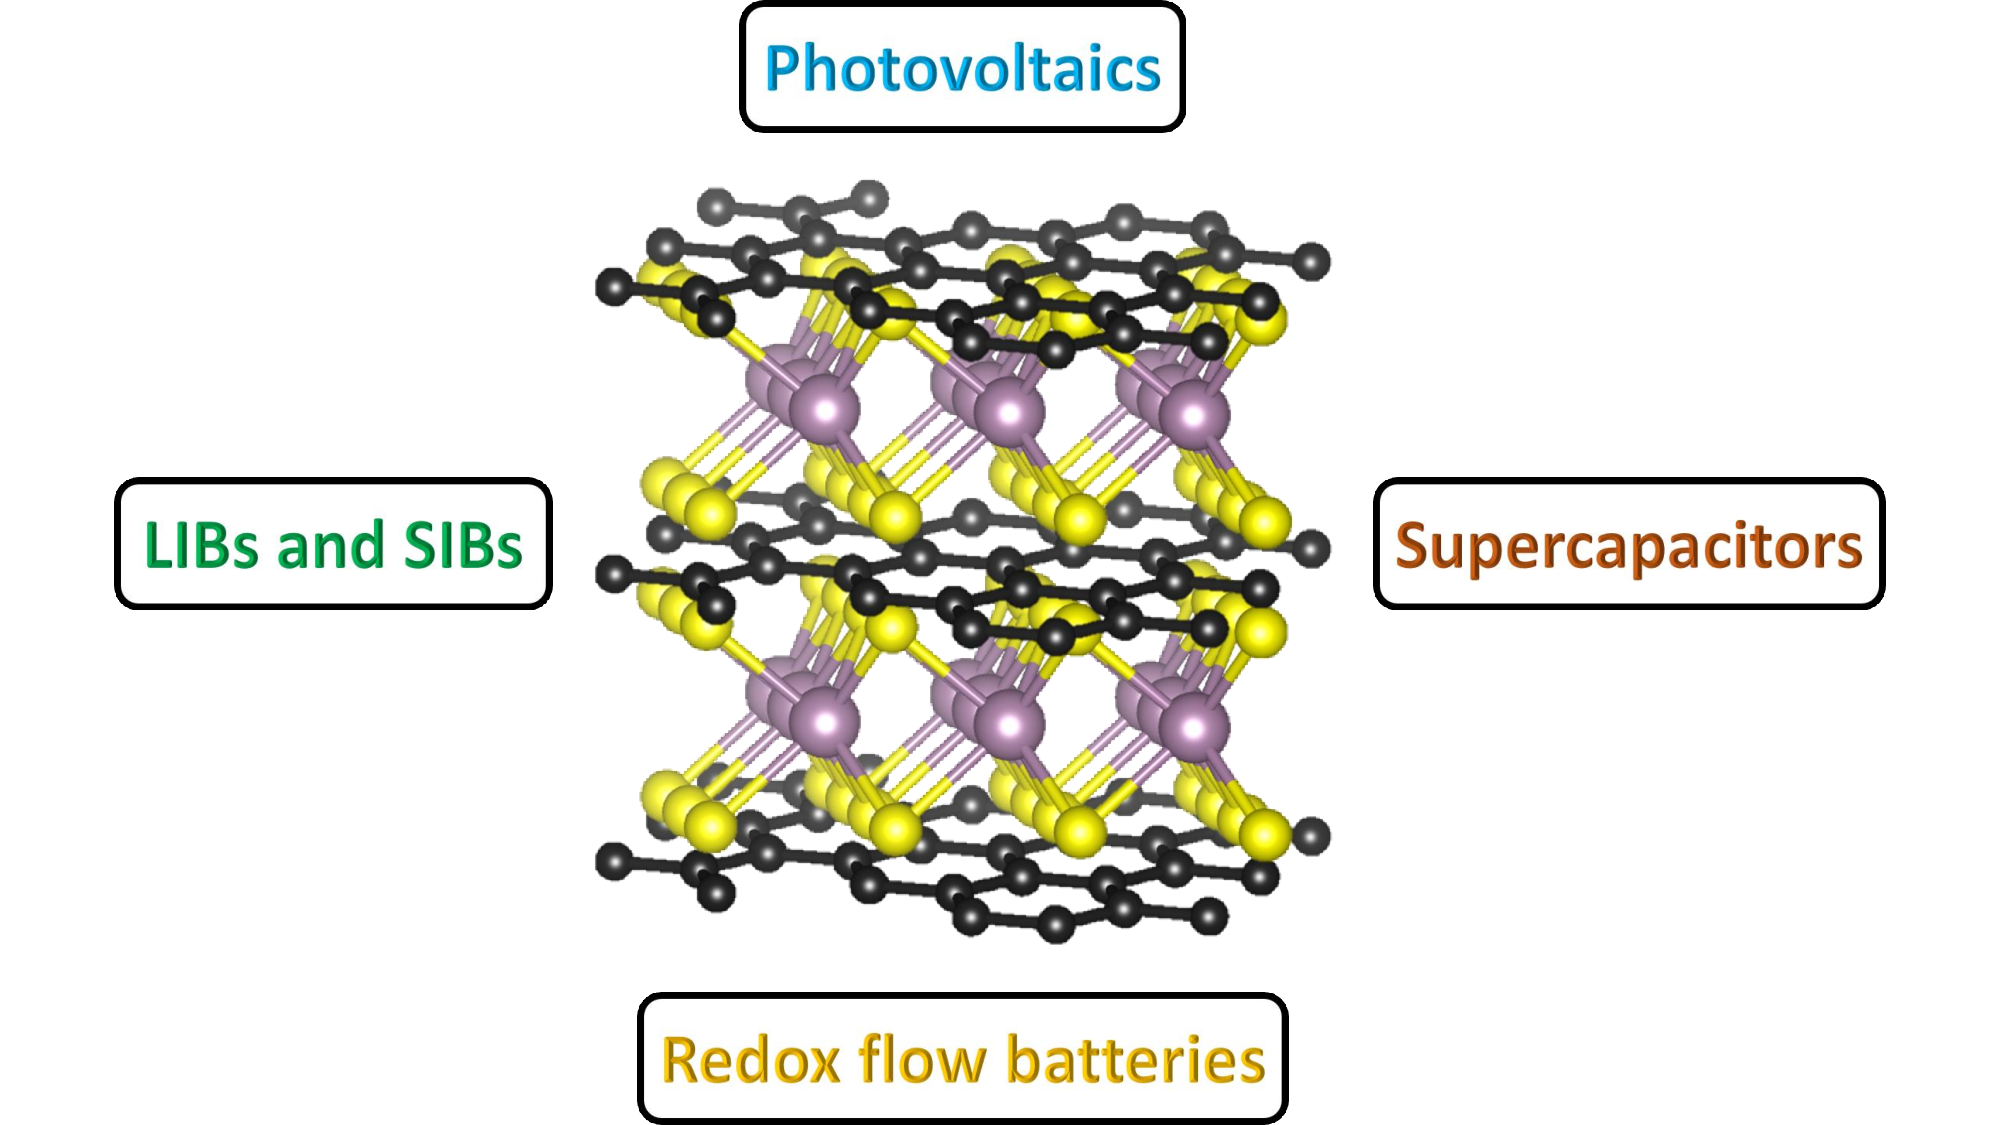
\includegraphics[width=\textwidth]{Figures/chap6fig/nanoTMDintro.pdf}
    \caption{.}
  \label{Figures/chap6fig:nanoTMDintro}
\end{figure}

\section{Nano-structured molybdenum sulfide and selenide}
Some TMDs such as \ce{TiS2} and exfoliated \ce{MoS2} flakes exhibit fast ionic conductivity as an electrochemically active material \cite{du_superior_2010,whittingham_electrical_1976}. A $\sim$750mAh g$^{-1}$ specific capacity was reported for restacked \ce{MoS2} single layers as a lithium-ion battery electrode. The restacking enlarged the c-axis parameter—the interlayer spacing, which increased the accessible surface area \cite{ammundsen_novel_2001}.
\subsection{Introduction}
Nano-sized materials increase the contact area between an electrode and electrolyte. The materials provide short path lengths for both ion diffusion and electron transport in comparison with bulk particles, which enhances the charge/ discharge rate. Since a shorter path length for electronic transport is created, materials having low electronic conductivity can also be utilised \cite{pitchai_nanostructured_2011}. The high surface area of nanomaterials allows large volume expansion/ contraction associated with ion transport and prevents cathode pulverisation, which leads to a longer cycle-life \cite{zhang_ultrathin_2015, cong_intrinsic_2015}. Transition metal dichalcogenides (TMDs) have a high surface area and potential to undergo redox reactions because they have multiple valencies. Nano TMDs have been widely explored as electrode materials since they have the potential to improve the electrochemical performance.  \\*
Nano TMDs have excellent electrochemical properties with a high surface-to-volume ratio. These materials have shown some remarkable performances in LIBs, sodium-ion batteries (SIBs), lithium-sulphur (Li-S) batteries, magnesium-ion batteries (MIBs), etc. In LIBs, graphene sheets and its analogues have shown a larger capacity over a graphite anode. The electrodes made of nanomaterials provide several advantages over bulk electrodes such as a high surface area, large void spaces and good electrical stability, which improves their lithium storage capability. Sheets of transition metal oxides also exhibit high specific capacity, and good stability. They are abundantly available, and are relatively easy to prepare. The storage of \ce{Li+} ions is based on a conversion reaction, where a reversible redox reaction takes place between lithium and transition metal cations \cite{reddy_metal_2013}. TMOs such as \ce{Fe2O3}, \ce{V2O5}, \ce{Nb2O5} and \ce{TiO2} have been used as anodes in LIBs. Fe2O3, for example has a very high theoretical specific capacity of 1006 mAh g$^{-1}$. This is why TMDs and TMOs have been considered as the next generation of electrode materials in batteries. With the rapid progress in research on 2D nanomaterials, large-scale preparation of nano-structured materials at a low cost can be expected for practical applications in the near future. \\*

\begin{sidewaystable}
\centering
\caption{Summary of performances of 2D materials in various energy storage devices.} \label{table1}
\begin{tabular}{ |p{1.5cm}|p{3.5cm}|p{4.5cm}|p{4.5cm}|p{4.5cm}|}
 \hline 
\textbf{Ref.} & \textbf{Electrode} & \textbf{Electrolyte} & \textbf{Storage capacity} & \textbf{Cycle performance} \\ 
\hline
\cite{acerce_metallic_2015-1} & {\center{Metallic 1T \ce{MoS2}}} & 0.5M \ce{H2SO4}, \ce{Li2SO4}, \ce{K2SO4} or KCl or EMIm \ce{BF4} & Volumetric capacitance: 400-700 F cm$^{-3}$ & >90\% retained after 5000 cycles\\
\cite{zhao_flexible_2015} & MXene/CNTs & 1M \ce{MgSO4} & Volumetric capacitance: 350F cm$^{-1}$ & No degradation after 10000 cycles at 10 A g$^{-1}$\\
\cite{hu_hierarchical_2015} & \ce{TiO2} & 1M \ce{LiPF6} in a 1: (v:v) mixture of ethylene carbonate and dimethyl carbonate & Specific capacity: 182 mAh g$^{-1}$ at 5C & 87.9\% retained after 400 cycles at 5C \\
\cite{cao_preparation_2013} & \ce{MoS2}/graphene & 1M \ce{LiPF6} in a 1:1 (V:v) mix of ethylene carbonate and dimethyl carbonate & Specific capacity: 466 mAh g$^{-1}$ at 4 A g$^{-1}$ & 566 mAh g$^{-1}$ retained after 50 cycles at 0.5 A g$^{-1}$ \\
\cite{ding_facile_2012} & \ce{TiO2}/CNT \ce{SnO2}/CNT & 1M \ce{LiPF6} in a 1:1 (w:w) mix of ethylene carbonate and dimethyl carbonate & Specific capacity: 320 mAh g$^{-1}$ for \ce{TiO2}, 580 mAh g$^{-1}$ for \ce{SnO2} at 0.4 A g$^{-1}$ & 93.8\% retained after 120 cycles for \ce{TiO2}, 72.4\% retained after 40 cycles at 0.4 A g$^{-1}$ for \ce{SnO2}\\
\cite{xie_mos2/graphene_2015} & \ce{MoS2}/rGO & 1M \ce{NaClO4} in a 1:1 (V:v) mix of ethylene carbonate and dimethyl carbonate & Specific capacity: 350 mAh g$^{-1}$ at 0.64 A g$^{-1}$ & 227 mAh g$^{-1}$ retained after 300 cycles at 0.32 A g$^{-1}$ \\
\hline
\end{tabular}
\end{sidewaystable}

\subsection{Experimental methods}
The materials were obtained from Tohoku university and used as received. 
%Before adding sulfur, pristine \ce{MoO3} (Wako chemicals) was ball-milled for 4 hours. 1 mmol of ascorbic acid (Wako chemicals) as a reducing agent was dissolved in 5 ml of water and the mixture was magnetically stirred for at least 20 minutes under air. Subsequently, 1 mmol of S powder (Sigma-Aldrich) and 0.3 mmol of ball-milled \ce{MoO3} were placed in the reactor. Lastly, 5 ml of ascorbic acid aqueous solution was injected into the reactor vessels containing the powder mixture. The sealed reactor was kept at 400$^{\circ}$C in a tube furnace for 30 minutes. After heating, the samples were collected in the same procedure as above.

\subsection{Results and discussion}
\ce{MoS2} and \ce{MoSe2} nanoflowers achieved a discharge capacity of 55 mAh g$^{-1}$ and 65 mAh g$^{-1}$ at a current rate of 50 mA g$^{-1}$ respectively. Figure \ref{Figures/chap6fig:MoX2YNCDCsCEs}a and b shows the charge and discharge curves at different current rates ranging from 50 to 1500 mA g$^{-1}$ with cutoff voltages at 0.2 and 2.35 V. Figure \ref{Figures/chap6fig:MoX2YNCDCsCEs}c and d displays the rate performance of both cells. It was observed that at higher current, the capacity of the cell decreased, while the coulombic efficiency increased. At 1500 mA g$^{-1}$, both Al/\ce{MoS2} and Al/\ce{MoSe2} displayed a capacity of $\sim$20 mAh g$^{-1}$ with 99.5\% coulombic efficiency. The discharge capacity increased to 50 mAh g$^{-1}$ after 120 cycles at a slower current rate of 50 mA g$^{-1}$. However, it was observed that the discharge curve for both nano-structured cathodes was a smooth line without any plateaus or bends. If we recall Chapter\ref{chap4} (Figure \ref{Figures/chap4fig:MoX2CDCCV}), bulk molybdenum dichalcogenides showed distinct voltage bends and plateaus. It seemed that the electron transfer process was a surface-based adsorption and not an intercalation process. Since both \ce{MoS2} and \ce{MoSe2} nanoflowers display similar specific capacities at similar current rates after 120 cycles, it can be assumed that the chloroaluminates were reversibly adsorbed on their surface. 

\begin{figure}[h!]
  \centering
  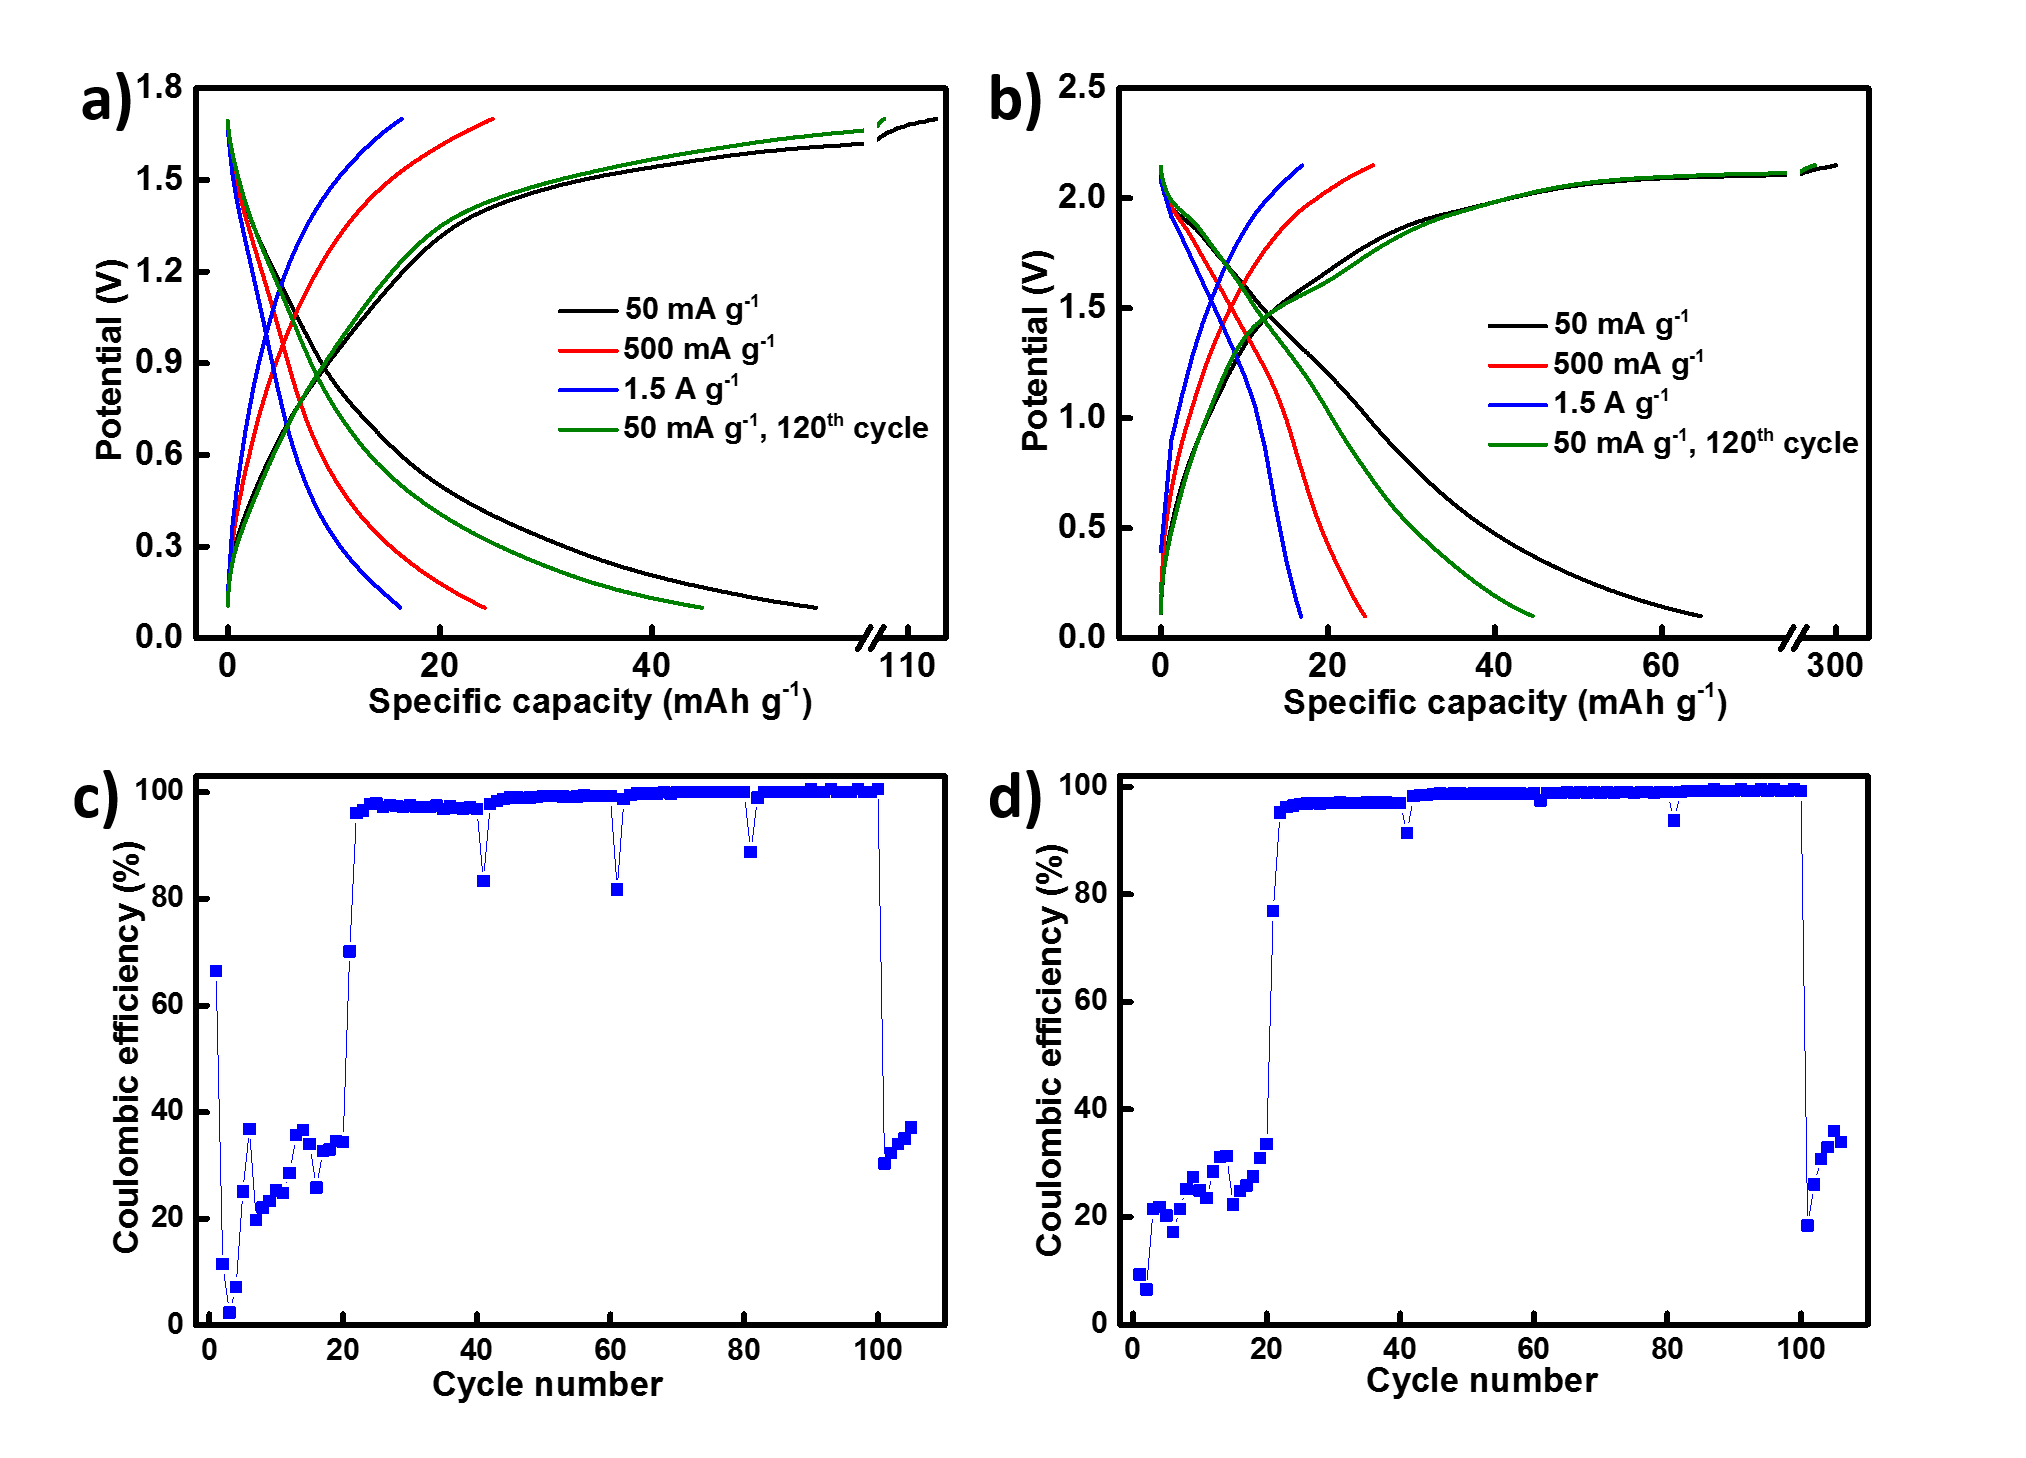
\includegraphics[width=\textwidth]{Figures/chap6fig/MoX2YNCDCsCEs}
    \caption{Galvanostatic charge and discharge curves of a) Al/\ce{MoS2} and b) \ce{MoSe2} cell at various current densities. Long-term stability test of c) Al/\ce{MoS2} and d) \ce{MoSe2} cells. All capacity was recorded between charging and discharging voltages of 0.2 and 2.35 V.}
  \label{Figures/chap6fig:MoX2YNCDCsCEs}
\end{figure}

\begin{figure}[th!]
\centering

\includegraphics[width=0.75\textwidth]{Figures/chap6fig/MoSe2YNCV}
\caption{\textit{Ex-situ} X-ray diffraction patterns of \ce{SnO2} cathode in a pristine (black), charged (green) and discharged (red) state.}
\label{Figures/chap6fig:MoSe2YNCV}
\end{figure}
Another interesting observation was the CV scan of nano-\ce{MoSe2}. The bulk and nano \ce{MoSe2} displayed their oxidation and reduction peaks at similar voltages. 

A schematic of the mechanism is displayed in Figure \ref{Figures/chap6fig:nanbulkmox2}.    

\begin{figure}[h!]
  \centering
  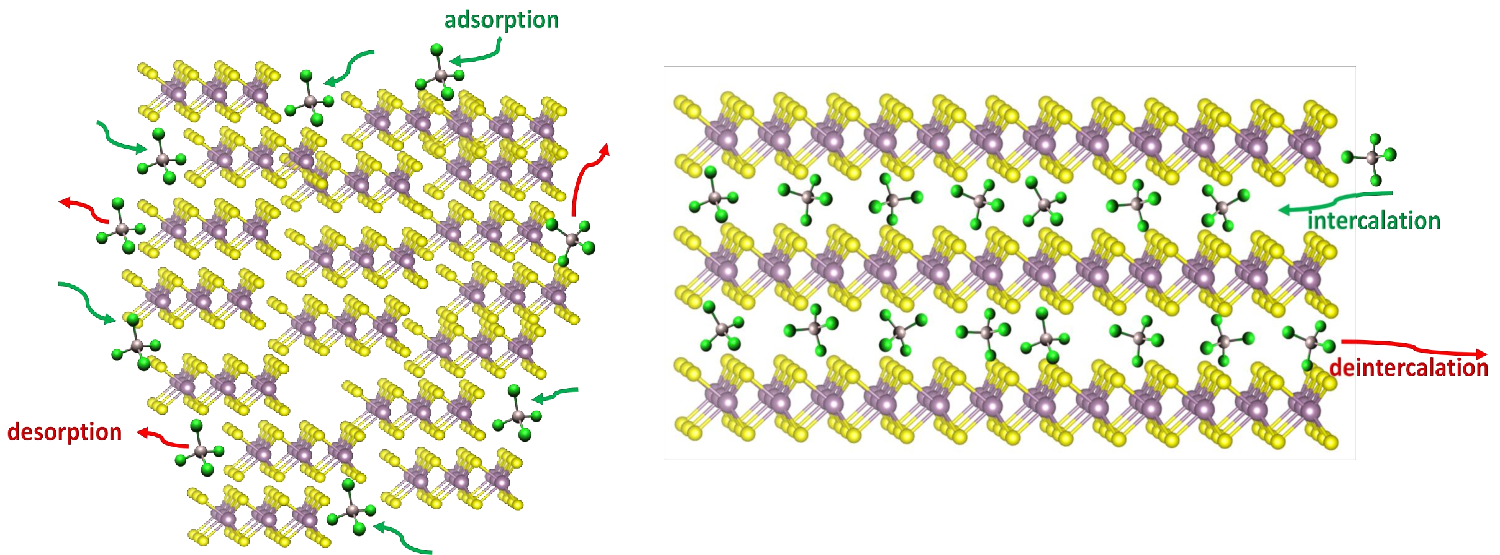
\includegraphics[width=\textwidth]{Figures/chap6fig/nanbulkmox2.pdf}
    \caption{Schematic illustration of the mechanisms followed by \ce{MoX2} nanoflowers (left) and bulk material (right).}
  \label{Figures/chap6fig:nanbulkmox2}
\end{figure}

While intercalation of chloroaluminates takes place in bulk \ce{MoX2}, the insertion of ions seems less probable on the nanoscale. Although the interlayer distance remains the same (6.5\AA) for both, the nano-sized structure obstructs a continuous intercalation process. Because of their high surface area, nanoflowers follow a capacitor-like charge storage, where the layers did not undergo any expansion and the specific capacities come from non-faradaic reactions where \ce{AlCl4-} anions electrostatically get absorbed and desorbed at their surfaces.

\section{Tin oxide}

\subsection{Introduction}

\begin{figure}[th!]
  \centering
  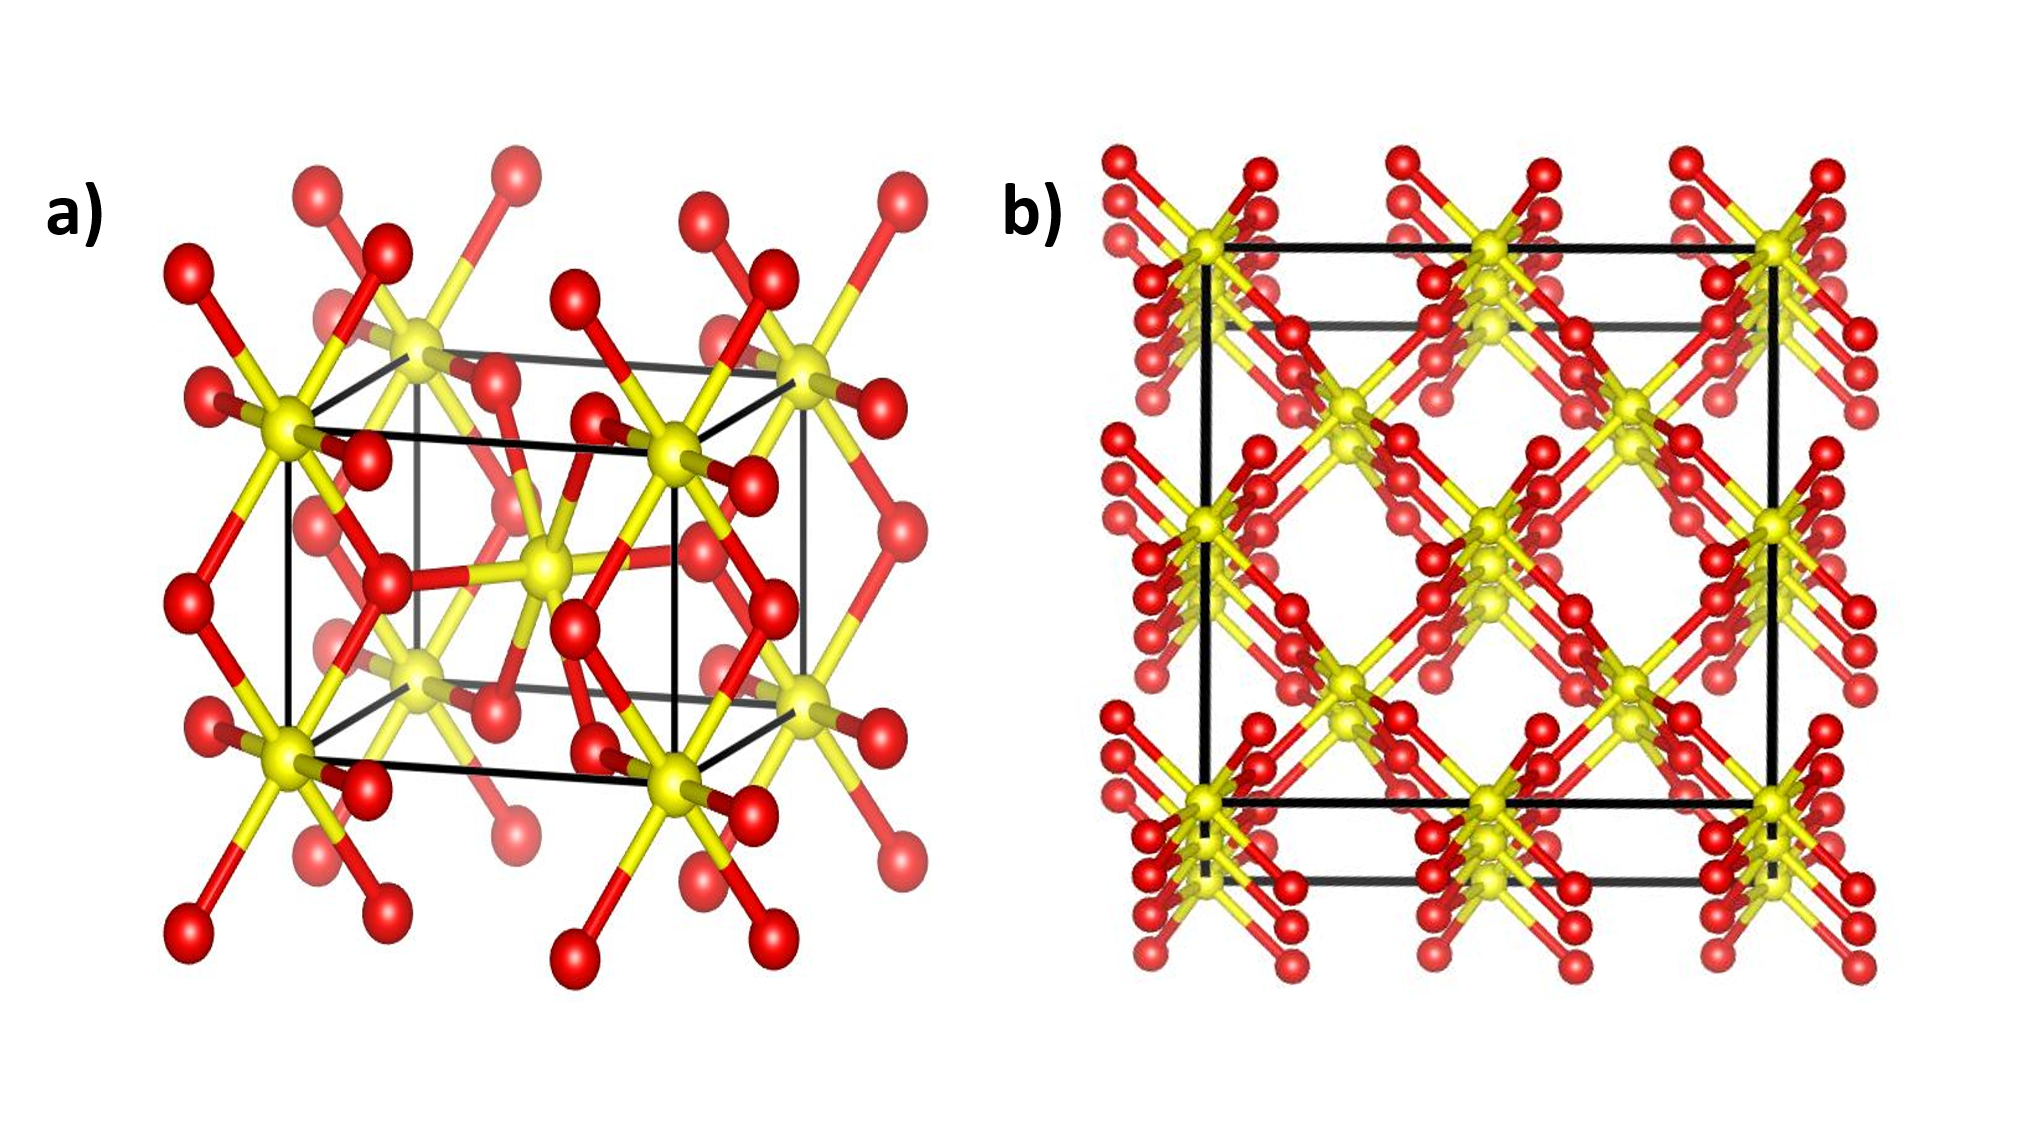
\includegraphics[width=\textwidth]{Figures/chap6fig/SnO2crys}
    \caption{Crystal structure of \ce{SnO2}. a) Tetragonal unit cell with space group P4/nmm and space group number 129. b) Top view of the crystal lattice.}
  \label{Figures/chap6fig:SnO2crys}
  \end{figure}
  
Due to its high theoretical capacity ($\approx$ 782mAh g$^{-1}$) and safe handling, \ce{SnO2} has been a popular choice in energy storage devices  \cite{idota_tin-based_1997}. They are a safer choice as compared to metallic lithium. Unfortunately, the major disadvantage of these materials is the large volume change during lithium insertion/extraction. A volume change of $\sim$360\% in pure tin metal causes an internal strain. Whittingham \textit{et al.} showed that pure tin foil (bulk) can be cycled as 600 mAh g$^{-1}$ for 10 to 15 cycles \cite{yang_anodes_2003}. However, the expansion and contraction of the anode during cycles causes pulverisation and increases of the cell impedance. Consequently, due to the loss of electronic contact between active materials and the current collector, the capacity of the cells decreases after 15 cycles. Formation of \ce{Li2O} in addition to the volume expansion, further deteriorates the battery performance \cite{zhao_tin-based_2016}. Equation 1 describes \ce{Li2O} formation and Equation 2 describes the large volume variation \cite{park_effect_2008}.

\begin{center}
\ce{SnO2} + 4\ce{Li+} + 4\ce{e-} $\longrightarrow$ 2\ce{Li2O} + \ce{Sn} (1) 
\end{center}
\begin{center}
x\ce{Li} + x\ce{e-} + y\ce{Sn} $\longrightarrow$ \ce{Li_{x}Sn}  (2)
\end{center}

Since \ce{Li2O} is electrochemically inactive and non-conductive, it is also responsible for the large initial irreversible capacity. It has been reported that \ce{Li2O} can be decomposed via structural modifications of \ce{SnO2} on a nanoscale. Tin-based anodes have demonstrated improved electrochemical performance and cycle life and a controlled expansion process during lithiation.  

\begin{figure}[th!]
\centering
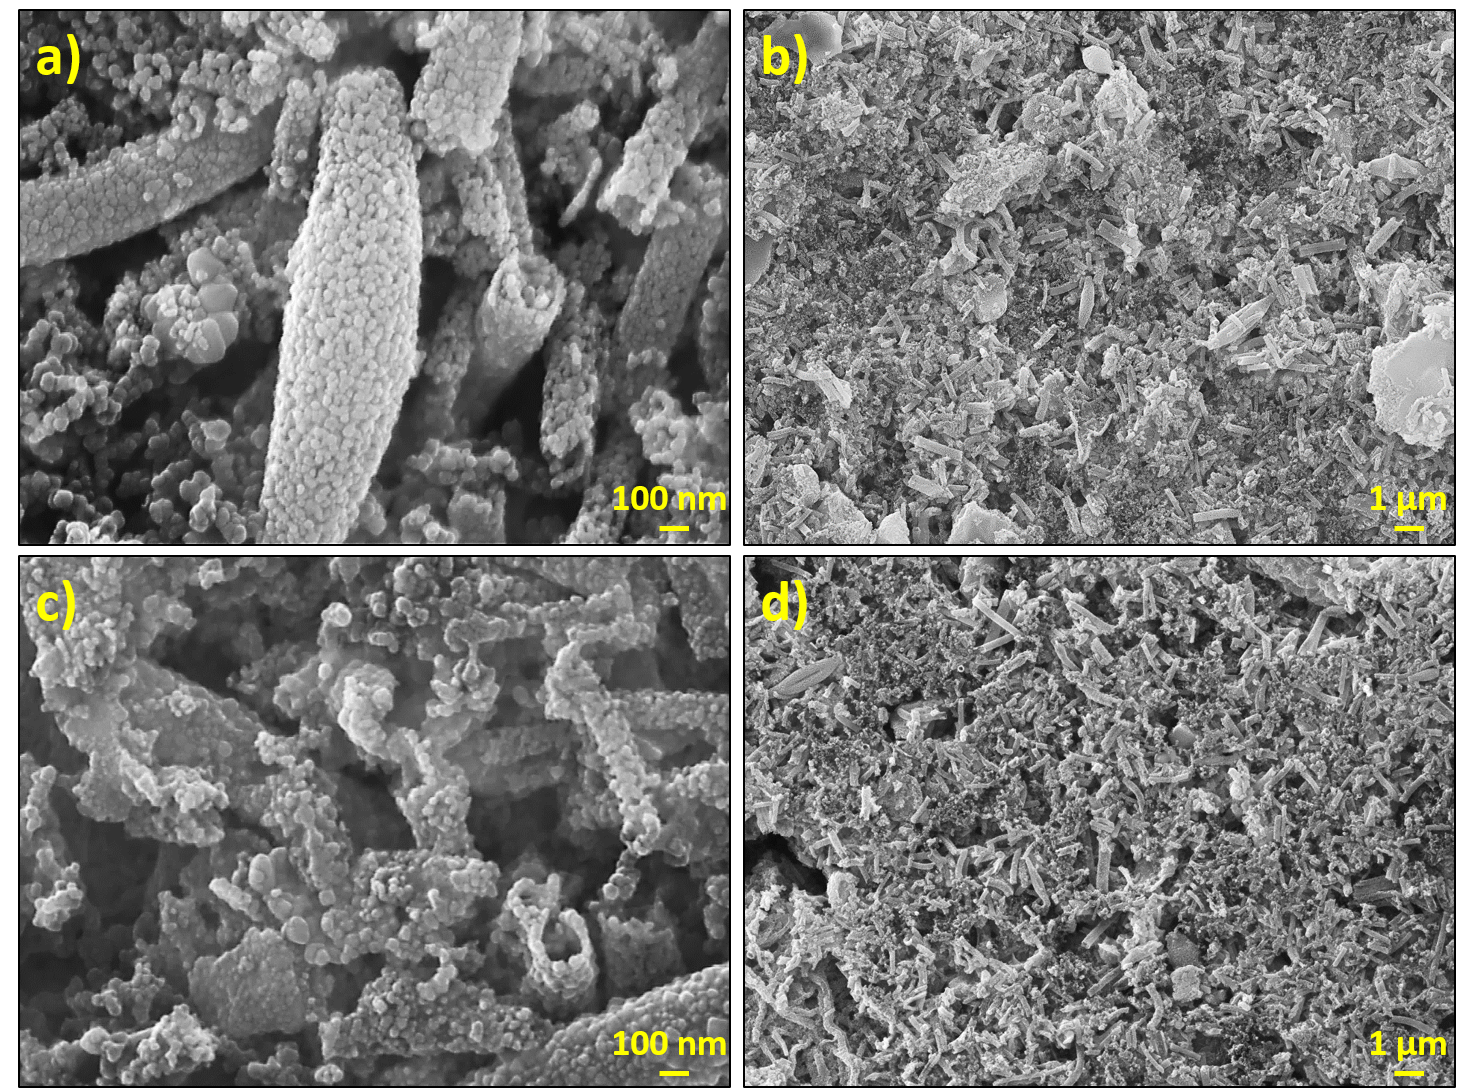
\includegraphics[width=\textwidth]{Figures/chap6fig/SnO2SEM}
\caption{SEM images of a,c)pristine and b,d) cycled \ce{SnO2} cathode.}
\label{Figures/chap6fig:SnO2SEM}
\end{figure}

It has been proposed that adding carbonaceous materials to \ce{SnO2} increases its surface area, which makes more active sites available for lithiation \cite{navarro-suarez_2d_nodate}. It also controls the volume expansion/shrinkage. Furthermore, it improves the conductivity of the material \cite{nowak_composites_2018}. Several nano-structured tin-based materials such as nano-rods \cite{liu_direct_2009}, nano-belts \cite{duan_single_2005}, nano-wires \cite{huang_situ_2010}, nano-tubes \cite{wang_large-scale_2011} have been synthesised and tested as electrodes. In this chapter, \ce{SnO2} fibers were obtained via  \enquote{electrospinning}. Electrospinning is a technique that uses electric force to draw charged threads of polymer solutions in the order of a few 100 nanometers. A schematic is illustrated in Figure \ref{Figures/chap6fig:electrospinning}. The topography and orientation of the fibers can be controlled by modifying a few parameters such as voltage, pump speed, nozzle thickness, etc. 

\begin{figure}[th!]
\centering
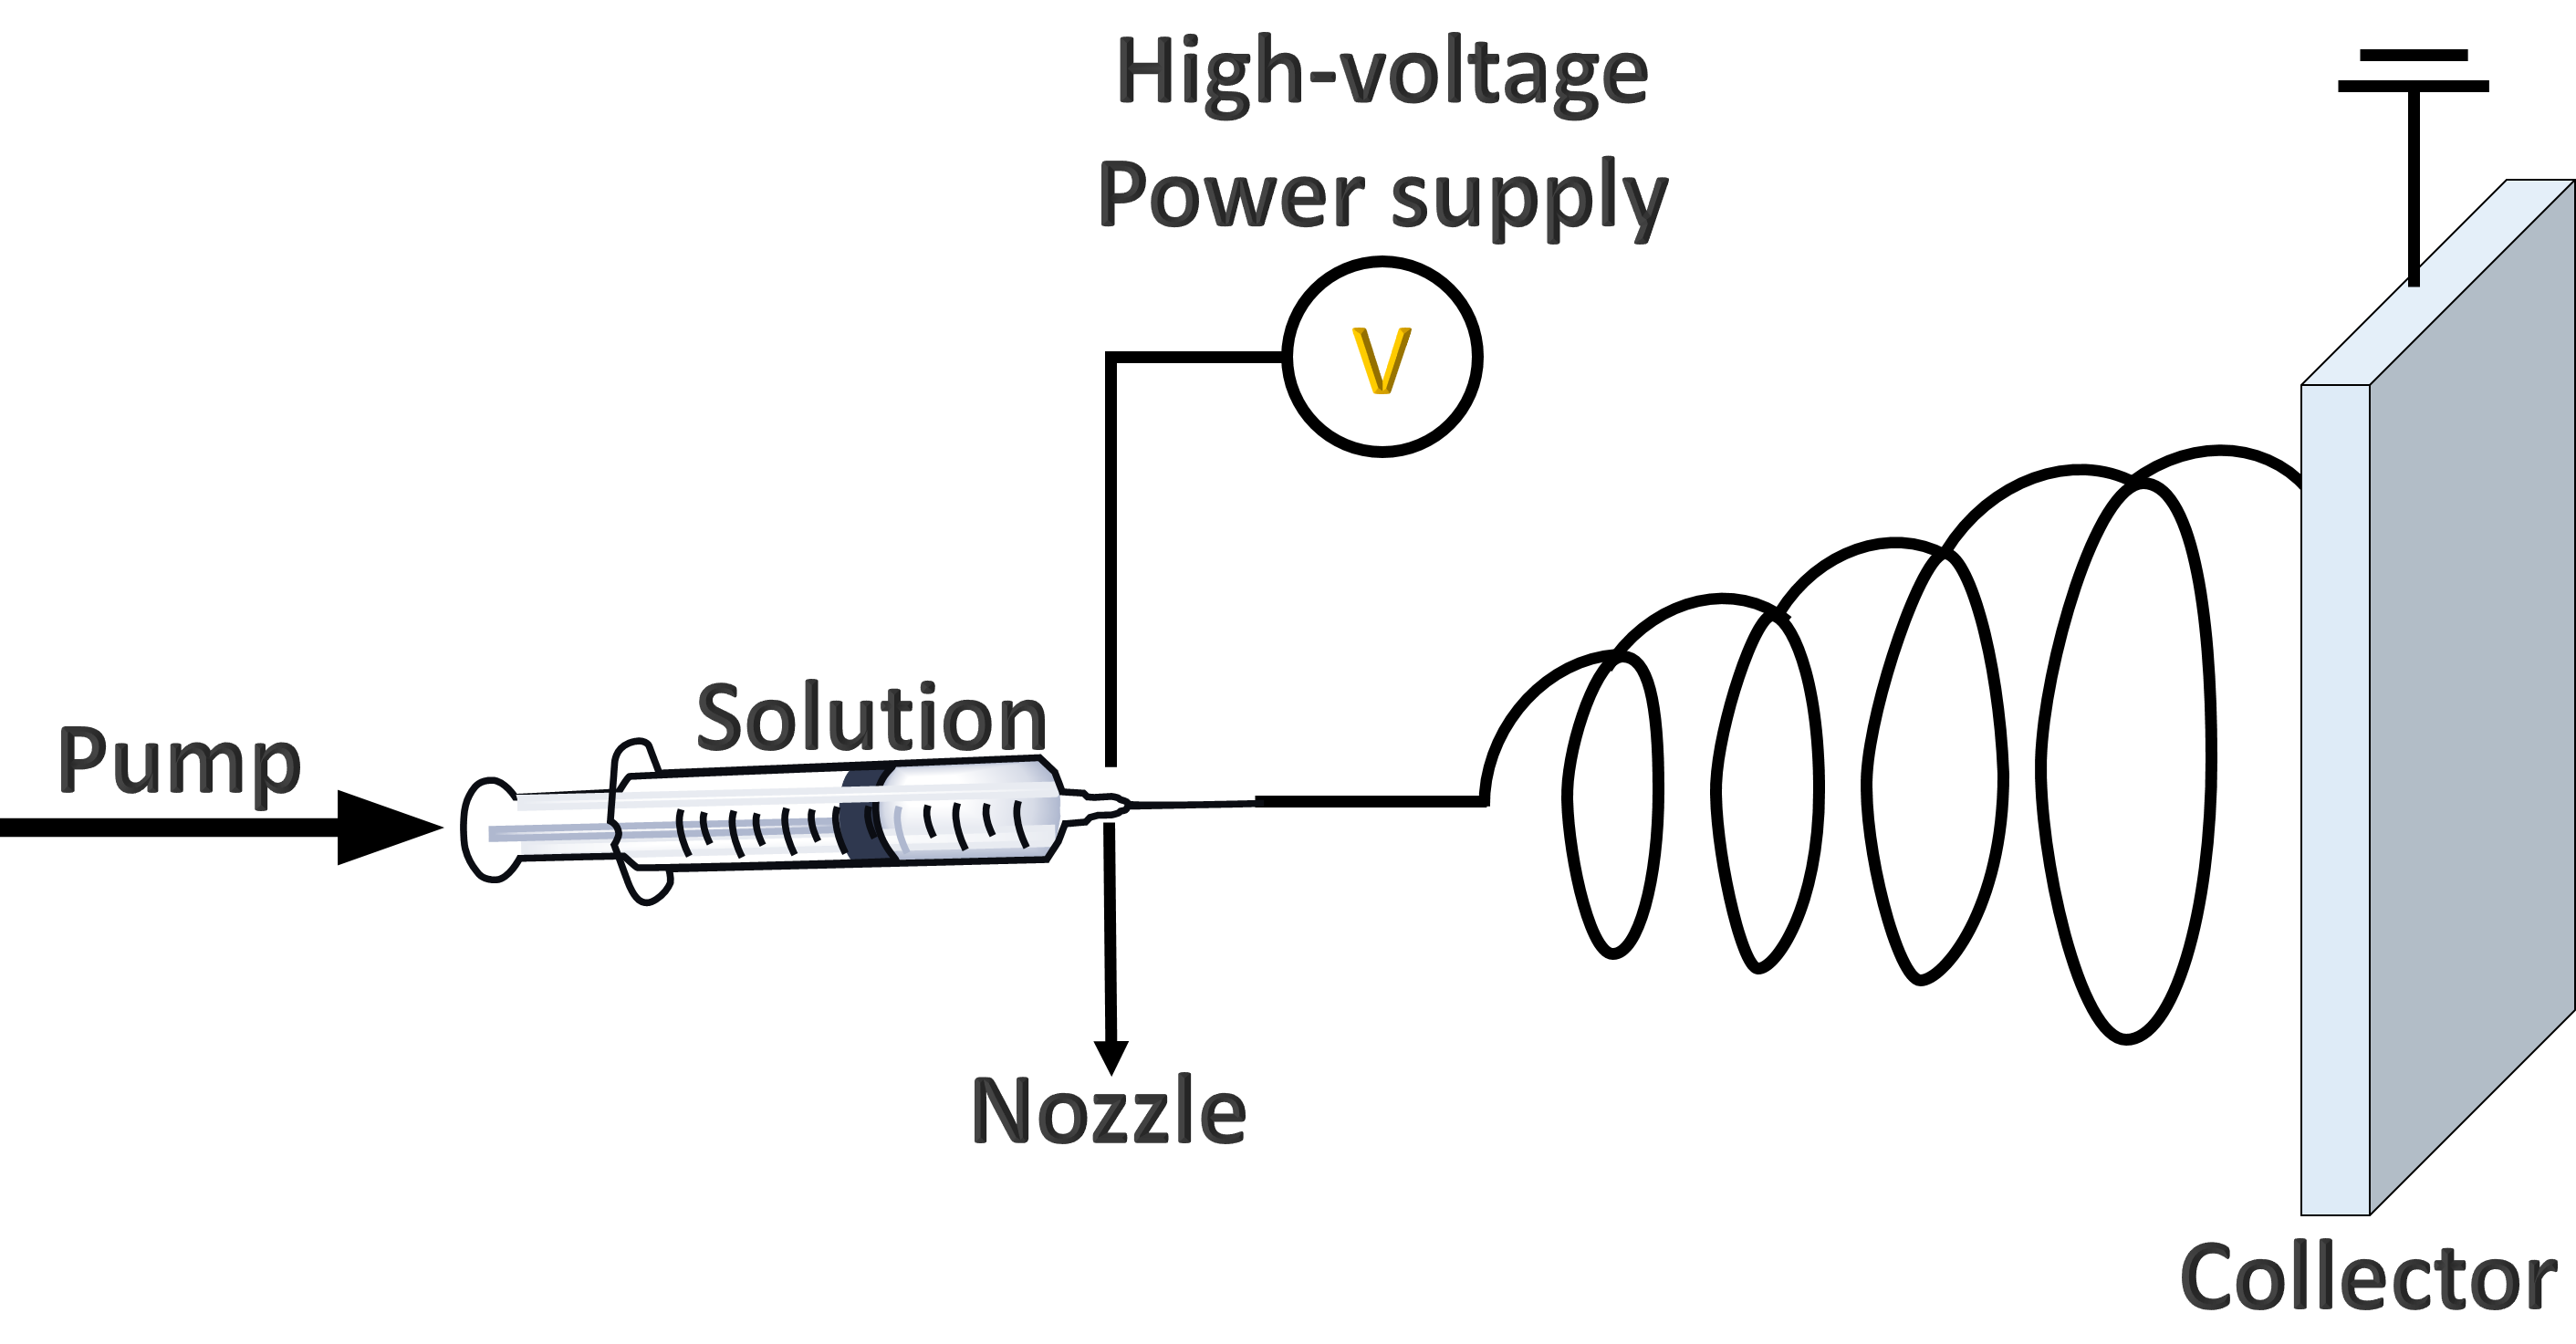
\includegraphics[width=\textwidth]{Figures/chap6fig/electrospinning}
\caption{SEM images of a,c)pristine and b,d) cycled \ce{SnO2} cathode.}
\label{Figures/chap6fig:electrospinning}
\end{figure}

\subsection{Experimental methods}
The material was obtained from University of Montpellier, France and was used as received. 

\subsection{Results and discussion}
To evaluate the electrochemical properties of the designed Al-ion cell, a galvanostatic discharge/charge reaction was performed at the cell voltage of 0.2-2.35 V at current densities ranging from 50-1500 mA g$^{-1}$. Figure \ref{Figures/chap6fig:SnO2newCDC} displays the voltage vs. specific capacity plot of the AIB. The curves demonstrate a well defined discharge plateau at $\sim$ 0.55 V. In the first cycle, the battery achieved a capacity of 105 mAh g$^{-1}$, which decreased to 50 mAh g$^{-1}$ after 120 cycles. Coulombic efficiency of the cell decreased with every cycle. It stabilised at $\sim$60\%. Since the discharge capacity decreases after every cycle,\ce{SnO2} as a cathode material in an AIB probably undergoes similar volumetric changes like in LIBs.   

 \begin{figure}[th!]
  \centering
  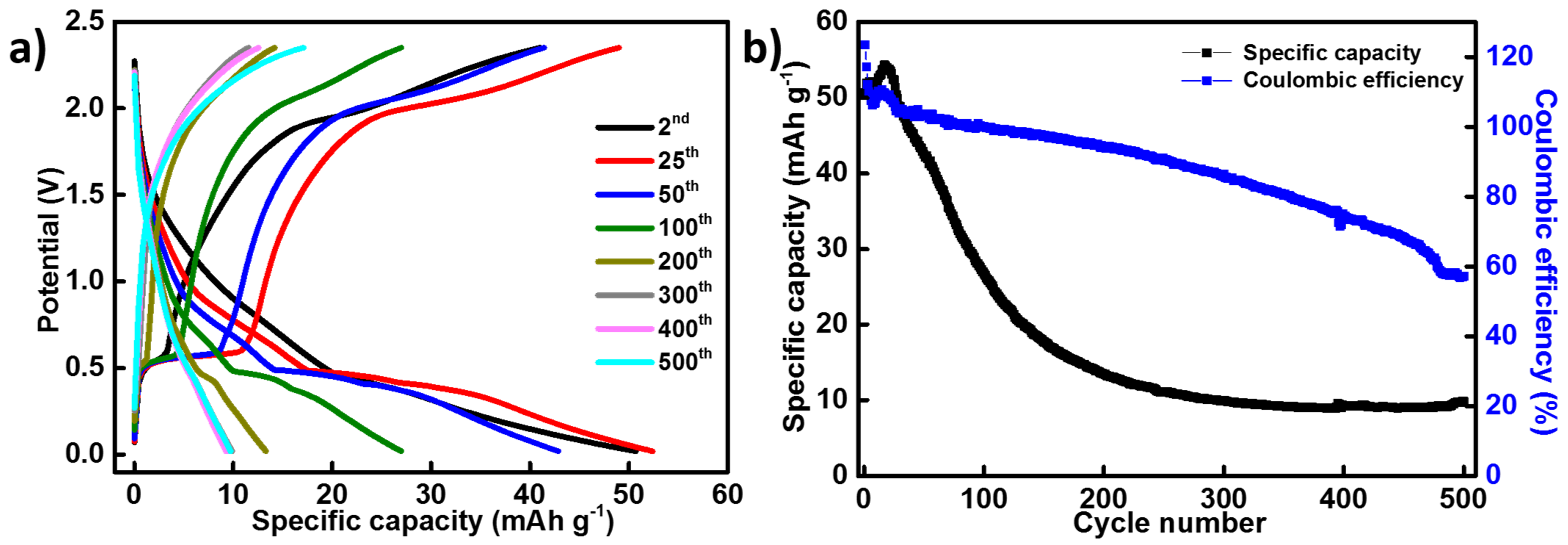
\includegraphics[width=\textwidth]{Figures/chap6fig/SnO2newCDC}
    \caption{Galvanostatic charge and discharge curve of an Al/\ce{SnO2} cell at various current rates.}
  \label{Figures/chap6fig:SnO2newCDC}
\end{figure}

\begin{figure}[th!]
\centering
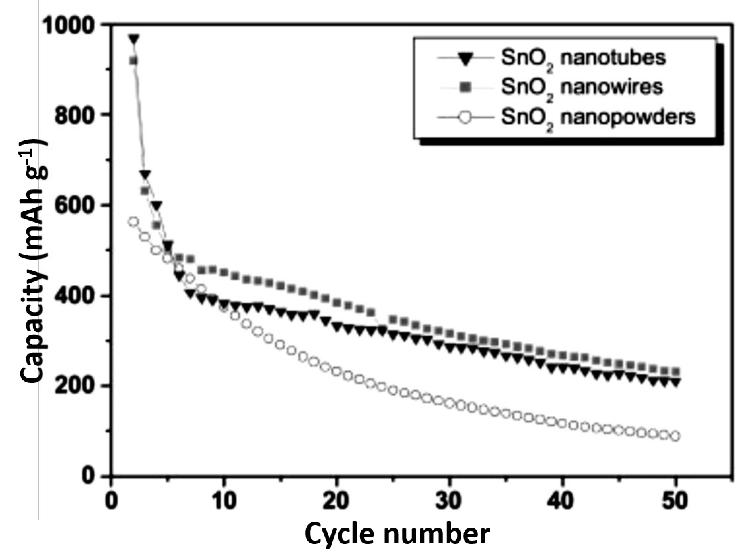
\includegraphics[width=0.75\textwidth]{Figures/chap6fig/sno2pap.pdf}
\caption{The cyclic performance of \ce{SnO2} nanomaterials in lithium-ion batteries up to the fiftieth cycle at a current density of 100 mA g$^{-1}$. Capacity of the materials decreases with every cycle due to expansion of \ce{SnO2}, which leads to cathode pulverisation and capacity fading.}
\label{Figures/chap6fig:sno2pap}
\end{figure}

However, the X-ray diffraction patterns in Figure \ref{Figures/chap6fig:SnO2XRD} look alike after charge and discharge except a shoulder that develops in the charged and discharged cathodes at 2$\theta$ value of 22$^{\circ}$. The fibers maintain their long-range order even after cycles. SEM images in Figure \ref{Figures/chap6fig:SnO2SEM} display the cathode morphology before and after cycles. The fibers seem to retain their tubular structure after charge/discharge, although a few fibres show signs of damage in Figure \ref{Figures/chap6fig:SnO2SEM}c. Furthermore, distinct voltage plateaus during charge and discharge respectively, indicate redox activity. To confirm the redox activity, cyclic voltammetry was performed and the resultant scans are displayed in Figure \ref{Figures/chap6fig:Sno2CV}. The CV exhibits a reduction peak at 0.45 V and an oxidation peak at 0.55 V, which correspond to the discharging voltage plateau at 0.47 V and charging voltage plateau at 0.55 V. 

 \begin{figure}[th!]
  \centering
  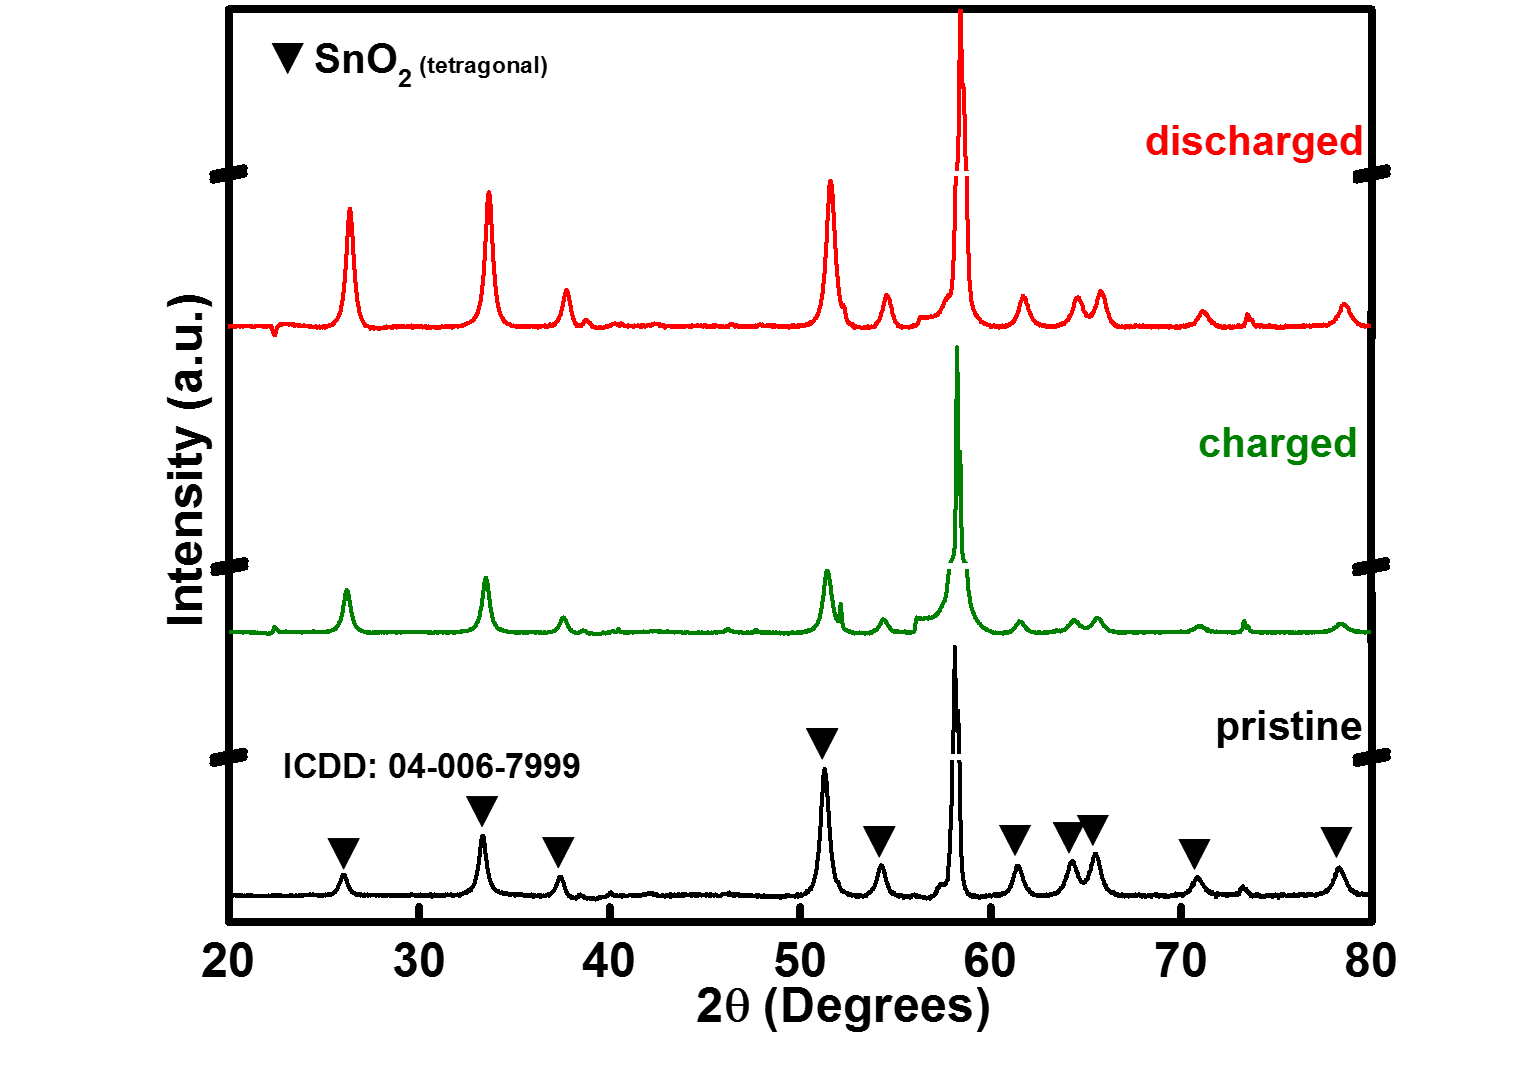
\includegraphics[width=\textwidth]{Figures/chap6fig/SnO2XRD}
    \caption{\textit{Ex-situ} X-ray diffraction patterns of \ce{SnO2} cathode in a pristine (black), charged (green) and discharged (red) state.}
  \label{Figures/chap6fig:SnO2XRD}
\end{figure}

 \begin{figure}[th!]
  \centering
  
\includegraphics[width=\textwidth]{Figures/chap6fig/Sno2CV}
    \caption{\textit{Ex-situ} X-ray diffraction patterns of \ce{SnO2} cathode in a pristine (black), charged (green) and discharged (red) state.}
  \label{Figures/chap6fig:Sno2CV}
\end{figure}

Further analysis is needed to investigate the ongoing mechanism. An \textit{ex-situ} XPS analysis of the charged and discharged cathodes would give additional information about the changing oxidation states of the active material at the redox potentials.


\section{Molybdenum trioxide}

\subsection{Introduction}

 \begin{figure}[th!]
  \centering
  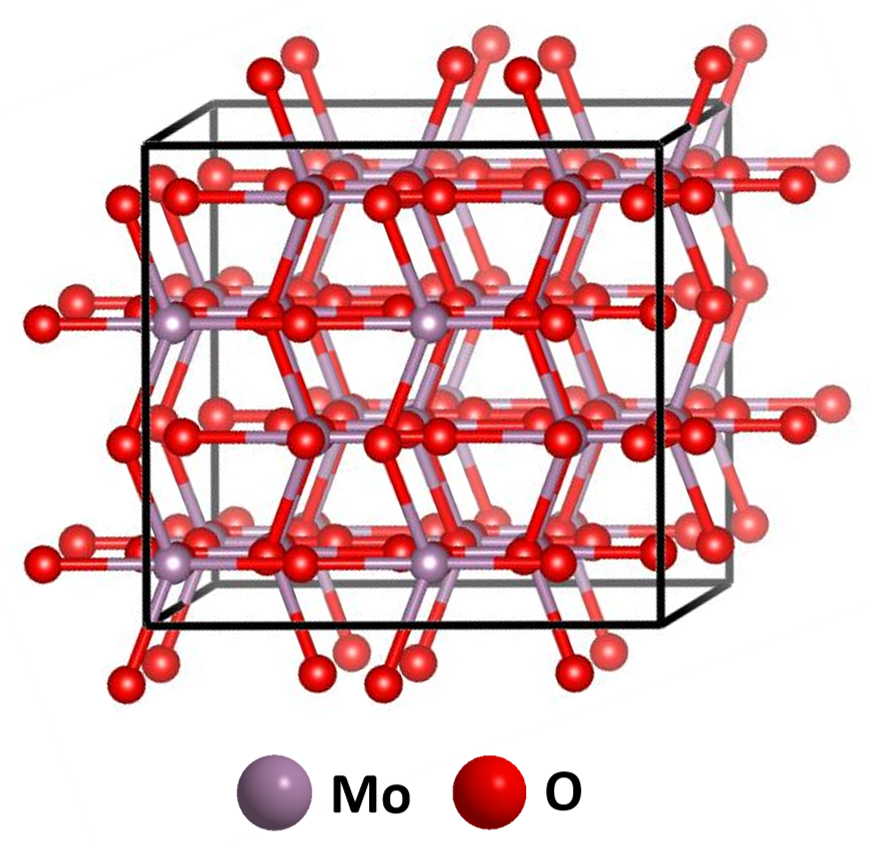
\includegraphics[width=\textwidth]{Figures/chap6fig/MoO3crys}
    \caption{Crystal structure of \ce{MoO3}. a) Tetragonal unit cell with space group P4/nmm and space group number 129. b) Top view of the crystal lattice.}
  \label{Figures/chap6fig:MoO3crys}
\end{figure}

Molybdenum trioxide, \ce{MoO3} is an intermediate formed during production of molybdenum metal. It has a layered orthorhombic arrangement with a space group of Pnma, and contains four formula units of \ce{MoO3} per unit cell. The single sheet adopts a bilayer structure with both sides of the surface terminated with oxygen atoms. The crystal structure of \ce{MoO3} is illustrated in Figure \ref{Figures/chap6fig:MoO3crys}. Due to its layered, \ce{MoO3} has been popularly used as an electrode material in LIBs \cite{wu_mixed_2017,li_vap,tsumura}. The intercalation of \ce{Li+} ions and the resulting redox reactions resulted in capacities ranging from 200-400 mAh g$^{-1}$ \cite{tsumura,chen_fast,zhou_-moo3_2010}. As one of the earliest studied host materials for \ce{Li+} insertion, $\alpha$ \ce{MoO3} can accommodate $\sim$ 1.5 lithium per Mo atom. Lithiated \ce{MoO3} (\ce{LixMoO3}) displayed good electronic conductivity and high \ce{Li+} mobility. It has been reported that the \ce{Li+} ions insert not only into the interlayer spacing between the \ce{MoO6} octahedron layers but also into the \ce{MoO6} intralayers \cite{li_vap,chen_fast}. However, high concentrations of unsolvated \ce{Li+} in the host lattice sometimes causes irreversible structural changes resulting in poor cell performance \cite{tao_moo3_2011,li_theoretical_2014}.\\
The reaction that takes place inside a LIB during discharge is given below. 

\begin{center}
    \ce{xLi+} + \ce{MoO3} + \ce{xe-} $\longrightarrow$ \ce{LixMoO3} \cite{li_vap}
\end{center}

The given reaction is reversed during discharge.

\ce{MoO3} has also been used as a cathode material in aqueous AIBs \cite{joseph_hexagonal, shakir_structural_2010, lahan_al3+_2019, lahan_active_2018}. Lahan and Das \textit{et al.} reported that intercalation of \ce{Al^{3+}} cations was possible in orthorhombic \ce{MoO3}. However the performance was dependent on the electrolyte composition. They demonstrated that with \ce{AlCl3}, the \ce{Al^{3+}} ion storage capacity of \ce{MoO3} increases as compared to \ce{Al2(SO4)_3} and Al\ce{(NO3)_3}. It also minimized polarization and improved the long-term stability of the cell. \ce{MoO3} cell achieved a specific capacity of 680 mAh g$^{-1}$ (highest reported value for any aqueous AIB) after its first discharge cycle. \\ 
Since \ce{MoO3} was never tested before as a cathode in non-aqueous AIBs, it was used as an active material during this project. However in 2018, Nacimiento \textit{et al.} used layered-type $\alpha$-\ce{MoO3} as a cathode in non-aqueous AIBs using \ce{AlCl3}:EMIC in the ratio of 1.1:1.0 (slightly acidic melt) as the electrolyte. However, the maximum capacity achieved was 100 mAh g$^{-1}$, which decreased to 85 mAh g$^{-1}$ after 7 cycles. In addition, a rapid capacity decay was observed. After 11 cycles, the capacity decreased to 40 mAh $^{-1}$ at a current rate of 3 mA g$^{-1}$. Due to all of the above-mentioned properties and advantages, \ce{MoO3} was used as a cathode material in an AIB. 

\begin{figure}[th!]
\centering
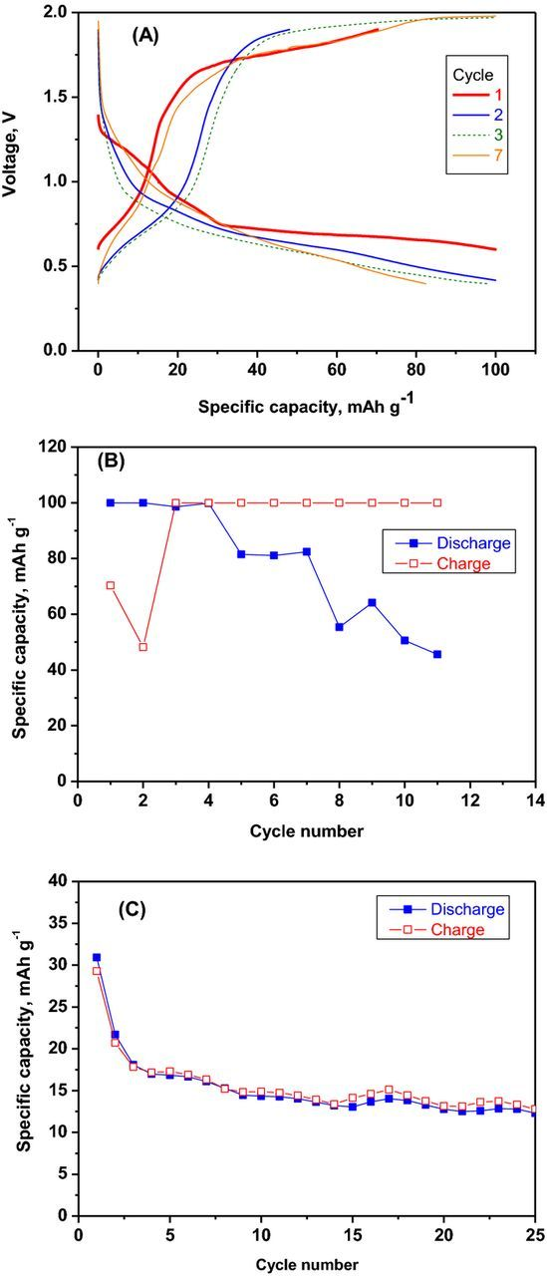
\includegraphics[width=\textwidth]{Figures/chap6fig/moo3pap}
\caption{Galvanostatic experiments for MoO3 in aluminum cell. A) Voltage-capacity curves and, B) corresponding capacity as a function of cycle number at current density 3 mA g$^{-1}$, and C) capacity as a function of cycle number at 10 mA g$^{-1}$ for 0.1-2.1 V of voltage limits.}
\label{Figures/chap6fig:moo3pap}
\end{figure}

\subsection{Experimental methods}
Molybdenum trioxide (\ce{MoO3} ACS reagent, $\geq$99.5\% was purchased from Sigma-Aldrich and used as received.

\subsection{Results and discussion}
At a high current density of 1500 mA g$^{-1}$ (Figure \ref{Figures/chap6fig:MoO3cdcce}a),\ce{MoO3} achieved the highest capacity of $\sim$80 mAh g$^{-1}$ with coulombic efficiency>100\% in its first cycle. After 120 cycles, the cell managed to retain 75\% of its original capacity. Voltage bends were observed at 2.0 and 1.7 V for the first 100 cycles. Plateaus were observed during charge and discharge at 2.0 and 1.4 V respectively. Discharge capacities at various current densities ranging from 50 mA g$^{-1}$ to 1500 mA g$^{-1}$ is shown in Figure \ref{Figures/chap6fig:MoO3cdcce}. Furthermore, this cell performed better than Nacimiento's cell with much higher cycle life and more stable diachrge capacities. 

\begin{figure}[th!]
\centering
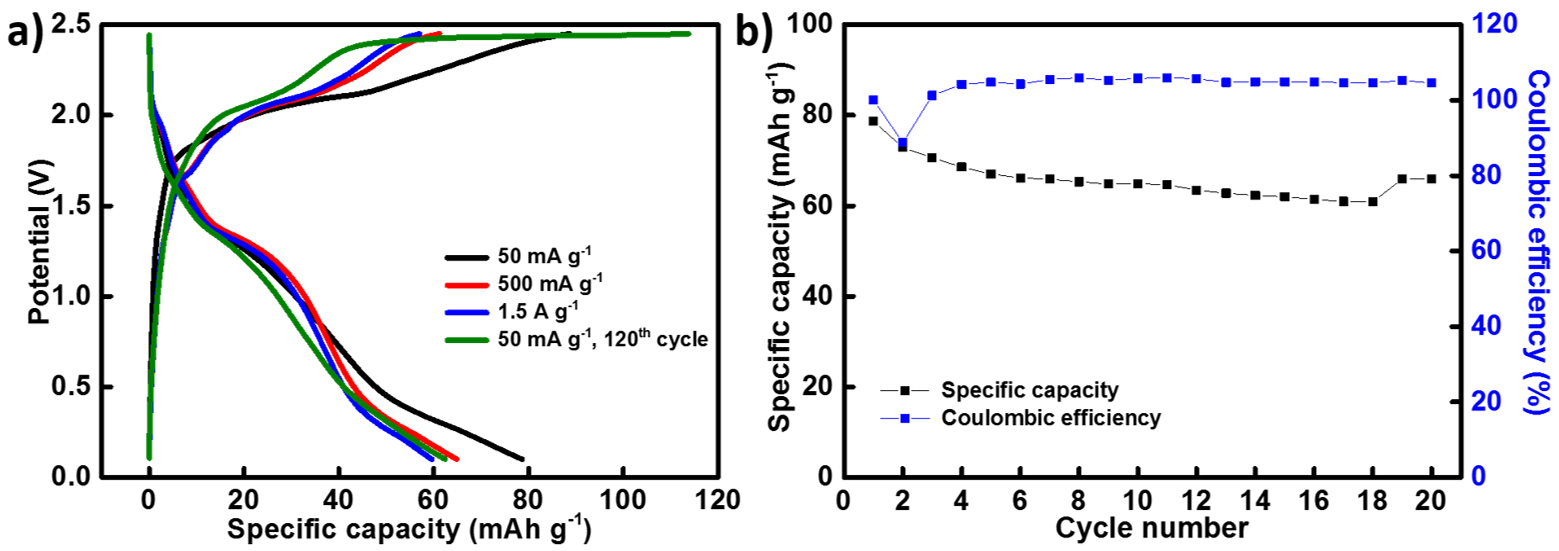
\includegraphics[width=\textwidth]{Figures/chap6fig/MoO3cdcce}
\caption{Charge/discharge cycles of an Al/\ce{MoO3} cell at various current rates.}
\label{Figures/chap6fig:MoO3cdcce}
\end{figure}

\subsection{Summary and conclusions}
\ce{MoO3} exhibited a capacity of 60 mAh g$^{-1}$ at 1500 mA g$^{-1}$ after 100 cycles, with clear charging/discharging plateau. This suggests fast intercalation-based redox reactions similar to what has been observed in LIBs. Advanced analytical techniques such as XRD or XPS would further support our hypothesis and establish its mechanism. With an energy density of $\sim$85 Wh kg$^{-1}$, this material shows a lot of potential for high-performing AIBs. 


\section{Graphitic Carbon Nitride}

\subsection{Introduction}
Graphitic carbon nitride or g-\ce{C3N4} is a carbon-based material that was first synthesised in 2012. The material is highly stable under physiological conditions and displays semiconductive properties. The crystal structure can be regarded as N-substituted graphite framework consisting of $\pi$-conjugated graphitic planes formed via sp$^2$ hybridisation of C and N atoms. The inter-layer distance between two stacks is 3.26\AA, and is 2\% more densely packed than crystalline graphite \cite{zheng_graphitic_2012}. Due to N-atom substitution, the binding between two layers is strengthened, which decreases its inter-layer distance. g-\ce{C3N4} is a low-cost metal free material with a high surface area. Since the structure of g-\ce{C3N4} is analogous to graphite, it has been used for electrochemical energy storage applications. \\*
g-\ce{C3N4} has been used as a battery electrode material in LIBs, Li-\ce{O2}, Li-S, Zn-air, vanadium redox flow batteries and sodium-ion batteries (SABs). The presence of pyridinic N in g-\ce{c3N4} favors high \ce{Li+} intake and prohibits irreversible reactions. Therefore, nitrogen content and its type, highly influence the performance of g-\ce{C3N4} in LIBs \cite{shah_highly_2017}. \\*
Vanadium redox flow batteries on the other hand, have also used g-\ce{C3N4} as a catalyst. A typical vanadium redox flow battery consists of two electrolyte tanks with \ce{VO2+}/\ce{VO^{2+}} and \ce{V3+}/\ce{V2+} redox couples, two pumps and a battery cell. The electrochemical reactions take place at the electrode. For this reason, highly efficient catalysts are a necessity. Huang \ce{et al.} modified carbon felt (usually used as a catalyst in flow batteries) with g-\ce{C3N4} for catalyzing the redox reactions. This increased the energy efficiency (EE) of the cells to 87\%. In addition, Nafion membranes were replaced by g-\ce{C3N4} hybrids, such as sulfonated poly(ether ether ketone) SPEEK/g-\ce{C3N4} and oxidised g-\ce{C3N4} (OCN) ion membranes \cite{niu_novel_2017, wang_novel_2017}. An ion membrane separates the ion-pairs in the flow battery and accelerates the proton flow during charge/discharge cycles. SPEEK/g-\ce{C3N4} showed a structure with roughness. The g-\ce{C3N4} modified membranes not only improved the EE of the flow batteries but also increased its coulombic efficiency (CE: 97\% and EE: 83.6\%) as compared to Nafion (CE: 90\% and EE: 73.8\%). A good structure stability against strong oxidizing and acidic condition was reported. The acid-base pairs formed between -\ce{NH2} groups of g-\ce{C3N4} and sulfonic acid groups of SPEEK enhanced the vanadium ion permeability and its selectivity, and also improved the proton transport channel \cite{wang_novel_2017}. SPEEK/OCN membranes due to their high surface area and intrinsic stability of OCN contributed to decrease the vanadium ion permeability. The functional groups of OCN helped in improving the proton conductivity and improved the battery's performance. Due to all of the above-mentioned properties and advantages, g-\ce{C3N4} was tested as a cathode material for non-aqueous AIBs. It was hypothesised that the chloroaluminate ions would undergo a similar intercalation-type process that would be supported by the graphitic framework.

\begin{figure}[th!]
\centering
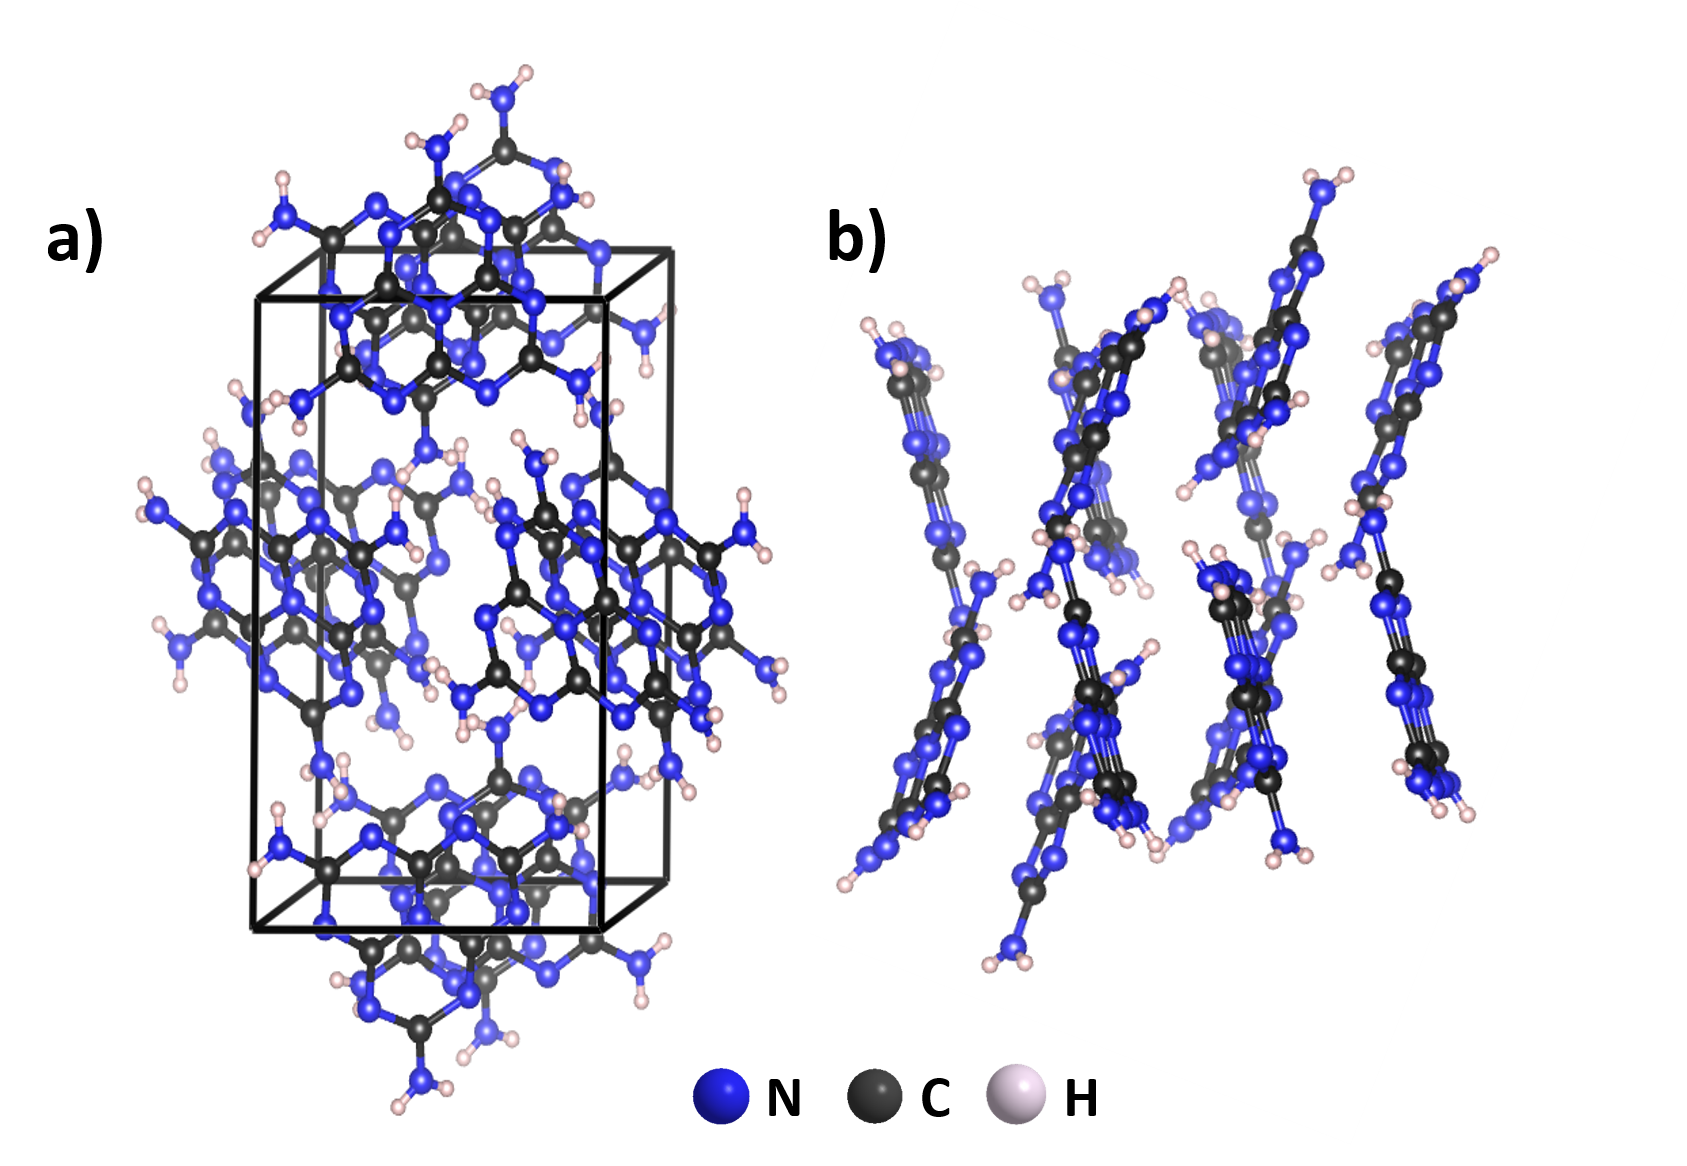
\includegraphics[width=\textwidth]{Figures/chap6fig/C3N4crys}
\caption{.}
\label{Figures/chap6fig:C3N4crys}
\end{figure}
\subsection{Experimental methods}
The material that was synthesised from urea was obtained from the University of Auckland and was used as received. 

\subsection{Results and discussion}
Figure \ref{Figures/chap6fig:C3N4cdc} shows charge/discharge curves and charge/discharge capacities of the rechargeable Al cell using g-\ce{C3N4} as the positive electrode. The discharge capacity at the first cycle was 100 mAh g$^{-1}$, which decreased to $\sim$80 mAh g$^{-1}$ after 120 cycles. Figure \ref{Figures/chap6fig:C3N4cdc}a shows the discharge capacities at current densities ranging from 50 mA g$^{-1}$ to 1500 mA g$^{-1}$. At 50 mA g$^{-1}$, the cell achieved a capacity of 100 mAh g$^{-1}$, which decreased to 20 mAh g$^{-1}$ at 1500 mA g$^{-1}$. The cell delivered a capacity of 95 mAh g$^{-1}$ at 500 mA g$^{-1}$, which proves that g-\ce{C3N4} has the ability to store charge even at higher current rates. A distinct charging plateau at 2.1V and a voltage bend during discharge at 0.6 V suggest towards redox activity. k

\begin{figure}[th!]
\centering
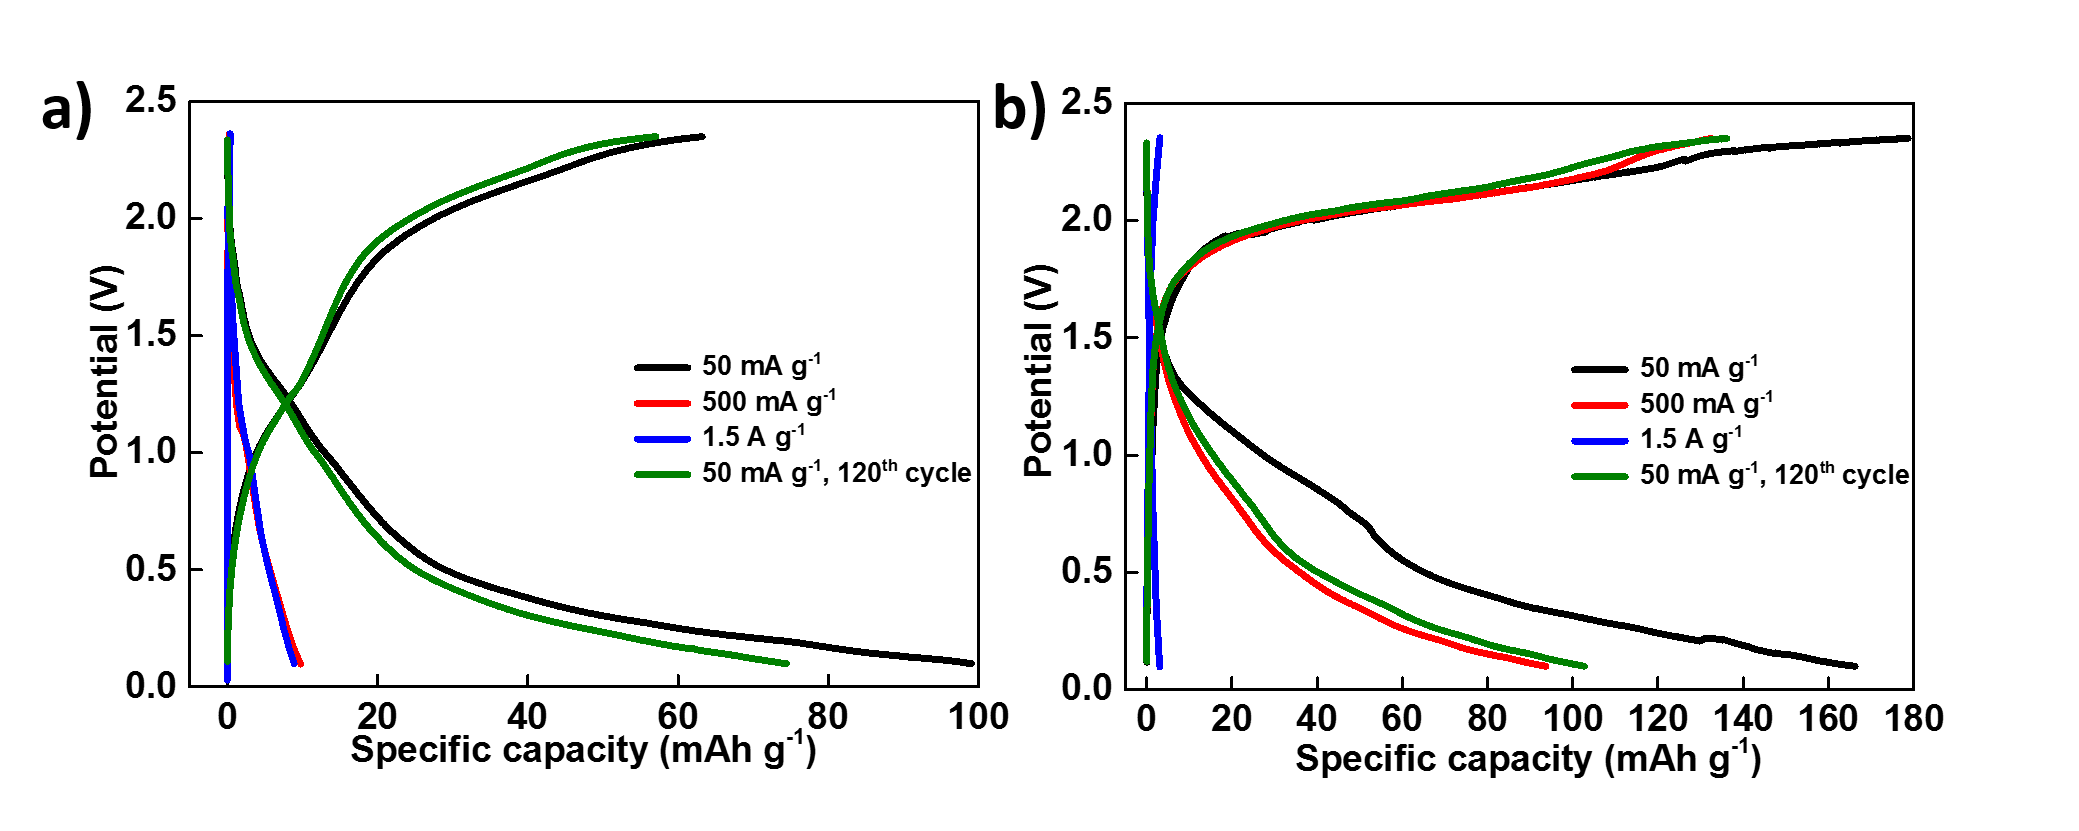
\includegraphics[width=\textwidth]{Figures/chap6fig/C3N4cdc}
\caption{Charge/discharge cycles of an Al/\ce{MoO3} cell at various current rates.}
\label{Figures/chap6fig:C3N4cdc}
\end{figure}

However, due to its chemical inertness, insolubility in most acidic, alkali and organic solvents, and low electronic conductivity, g-\ce{C3N4} needs to be explored further. However, its storage performance is largely affected due to its large contact resistance and low band-gap. Considerable efforts have been made to improve its performance for high-performing LIBs. Despite the fact that g-\ce{C3N4} has a more open structure than graphite, which should improve its \ce{Li+} intake and exchange capability, \cite{luo_graphitic_2019} \textit{et al.} showed that a LIB using g-\ce{C3N4} anode displayed a capacity of 134.9 mAh g$^{-1}$ only and an irreversible capacity loss of >98\% after 7 cycles. Veith and Hankel \textit{et al.} reported that reactions of lithium with g-\ce{C3N4} was responsible for the irreversible capacity loss \cite{veith_electrochemical_2013, hankel_lithium_2015}. Furthermore, replacement of C atoms with N atoms in the benzene ring was responsible for its poor conductivity. The above-mentioned reasons might also be the reason why the material did not retain its capacity when used as a cathode in the AIB. However, certain modifications can be made and new functional groups can be added to g-\ce{C3N4} that might improve its charge-storing capacity.

\section{Prussian blue}

\subsection{Introduction}

 \begin{figure}[tbh!]
  \centering
  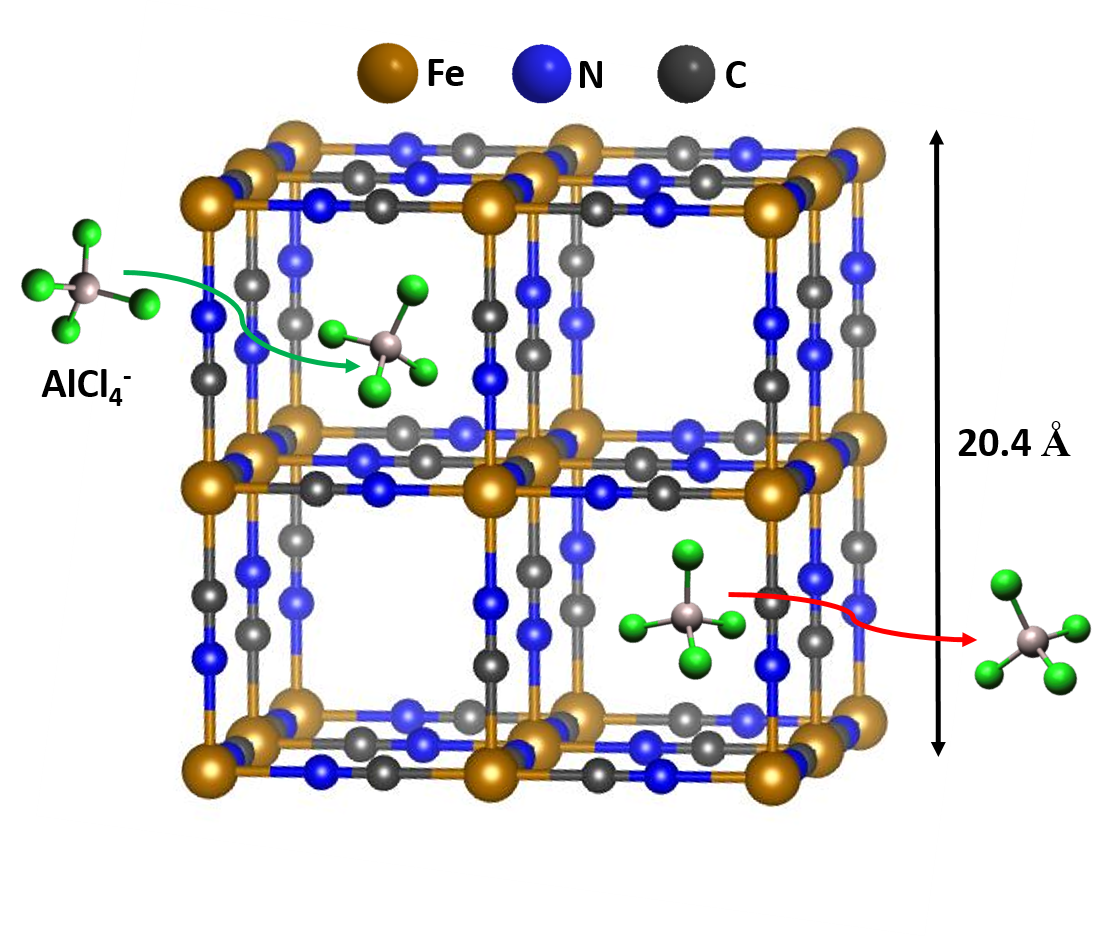
\includegraphics[width=\textwidth]{Figures/chap6fig/pbcrys}
    \caption{Crystal structure of Prussian blue a) Tetragonal unit cell with space group P4/nmm and space group number 129. b) Top view of the crystal lattice.}
  \label{Figures/chap6fig:pbcrys}
\end{figure}

Prussian blue belongs to the family of metal-organic framework, also known as MOF. A MOF is a hybrid crystalline porous material. It consists of a regular arrangement of positively charged metal ions and surrounded by organic molecules. A repeating cage-like structure is formed when metal cations form nodes that binds with an organic molecule's linker. MOFs have a large surface area (as high as 700 m$^{2}$g $^{-1}$) due to their hollow structure. Figure \ref{Figures/chap6fig:pbcrys} displays the crystal structure of Prussian Blue. The structural uniformity and and the flexibility in their network topology, makes MOF an ideal battery material. Its open framework allow insertion of ions in the sub-cages. The structure has a number of redox sites present as each molecular formula contains two redox centres \ce{M+2}/\ce{M3+}, where M is any transition metal (Fe, Co, Ni, Mn, Cu, Zn). It reaches 2\ce{e-} redox capacity after reversibly intercalating 2 monovalent alkali ions per molecular unit. Presence of large lattice interstices and ionic channels renders a high specific capacity. The ability to tune MOFs along with its structural design, makes it different from the conventional porous materials. Due to their high surface area and and tailored pore-size, MOFs have been utilised as electrode materials in electric double layer capacitors or EDLCs, LIBs and sodium-ion batteries. A Co-Zn MOF was designed by Diaz \textit{et al.} and it showed a typical EDLC behaviour in a non-aqueous electrolyte \cite{diaz_co8-mof-5_2012}. However, the specific capacitance for Co-Zn MOF was low. It was observed that cobalt-based MOF derived from Co\ce{(NO3)_2}, displayed pseudo-capacitance behaviour (presence of redox couples) instead of an EDLC behaviour with an improved specific capacitance. Lee \ce{et al.} observed a relationship between the pore size of MOFs and their performance in supercapacitors. After several attempts, it was determined that inclusion of conducting species within the MOF framework could solve the problem of low capacitance by providing an efficient electron pathway. Furthermore, MOFs with tailored channels or pores would allow faster diffusion of active ions during charge/ discharge cycles. The electrolyte also plays an important role in achieving high-performing supercapacitors. \\*
Recently, MOFs have been investigated as anode materials in LIBs \cite{li_shape-controlled_2006,han_synthesis_2012,zhao_metalorganic_2015}. To be used as anodes, the porous structure of MOFs allows reversible intercalation of \ce{Li+} ions during charge/discharge cycles. MOF-177 was the first MOF that was used as an anode material in LIBs \cite{}. The material underwent a conversion reaction inside the cell that destroyed its structure and consequently resulted in a poor cycling performance.  Zhang \textit{et al.} investigated Prussian blue nanoparticles as anodes \cite{nie_prussian_2014}. The open-framework structure allowed rapid intercalation/deintercalation of \ce{Li+} ions. The cell achieved a reversible capacity of 300 mAh g$^{-1}$ and superior rate capability. Yagi and his group studied the lithiation mechanism in Prussian blue and its analogues (PBAs) \cite{yagi_eqcm_2014}. They reported that the redox reaction of PB might also proceed with the electrochemical adsorption/ desorption of \ce{PF6-} ions, which are the counter ions in the electrolyte. MOFs have also been used as templates for preparing nano-structured metal oxides and and carbon materials. A few other MOFs used in LIBs as anode materials have been listed in Table \ref{tableMOF}. Th mechanism of \ce{Li+} storage in MOFs takes place via the following: \\*
\textbf{conversion reaction}: metal ions present in the MOF get replaced by \ce{Li+} ions \\*
\textbf{intercalation reaction}: \ce{Li+} ions get stored in the MOF's cage-like structure which keeps the structure intact \cite{wang_metalorganic_2016}. \\
MOFs have shown to have many applications in electrochemical energy storage. They can be used both in supercapacitors and in batteries. Based on the multiple valence of the metal ions, open framework and ligands with functionalities, novel electrode materials can be designed and used in AIBs. 

For all the above-mentioned properties and advantages, Prussian blue, a kind of MOF, was tested as a cathode material in this project. 

\vspace{0.5cm}
\begin{table}
\centering
\caption{Summary of performances of MOFs used as anode and cathode materials in various energy storage devices.} \label{tableMOF}
\begin{tabular}{ |p{1cm}|p{3.5cm}|p{2.2cm}|p{1.2cm}|p{1.5cm}|}
 \hline 
\textbf{Ref.} & \textbf{MOFs} & \textbf{Capacity (mAhg$^{-1}$)/ Capacitance (Fg$^{-1}$)} & \textbf{Voltage (V)} & \textbf{Surface area (m$^{2}$g$^{-1}$)} \\ 
\hline
\cite{li_shape-controlled_2006} & {MOF 177} & 425 & 0.1-1.6 & -\\
\cite{han_synthesis_2012} & Li/Ni-NTC & 1084 & 0.01-3 & -\\
\cite{zhao_metalorganic_2015} & Asp-Cu nanofibers & 1255 & 0.01-3 & -\\
\cite{wu_mof-templated_2013} & CuO & 1208 & 0.05-3 & -\\
\cite{huang_metal-organic_2014} & \ce{Fe2O3}/\ce{NiCo2O4} & 1311 & 0.01-3 & -\\
\cite{nagarathinam_redox-active_2012} & \ce{K2.5VO2}\ce{HPO4}\ce{C2O4} & 62 & 2.5-4.6 & -\\
\cite{zhang_monitoring_2014} & Cu(2,7-AQDC) & 147 & 1.7-4 & -\\
\cite{liu_metalorganic_2010} & NPC650 & 222 & - & 1521\\
\cite{hu_porous_2010} & MC-A & 208 & - & 1674\\
\cite{tang_thermal_2015} & NC/GC & 270 & - & 1276\\
\cite{chen_high-performance_2013} & N-PC & 219 & - & 484\\
\cite{banerjee_mof-derived_2014} & MOF-DC & 149 & - & 2714\\
\hline
\end{tabular}
\end{table}


\subsection{Experimental methods}
\subsection{Results and discussion}
The first charge–discharge curve exhibited distinct voltage bends and plateaus at 1.8, 1.2 V and 0.6 V with a capacity reaching $\sim$140 mAh g$^{-1}$ after first 20 cycles. To investigate the rate capabilities of the battery, the cell was charged and discharged at various current densities (Figure \ref{Figures/chap6fig:pbCDC2}a) ranging from 50-1500 mA g$^{-1}$. The specific capacities and coulombic efficiencies over 180 cycles at different current rates are shown in Figure \ref{Figures/chap6fig:pbCDC2}b. Discharge capacity after the first cycle is 140 mAh g$^{-1}$, and it exhibits multiple discharge voltage plateaus. With an increase in current density, the capacity of the battery gradually decreased to 5 mAh g$^{-1}$. 

 \begin{figure}[tbh!]
  \centering
  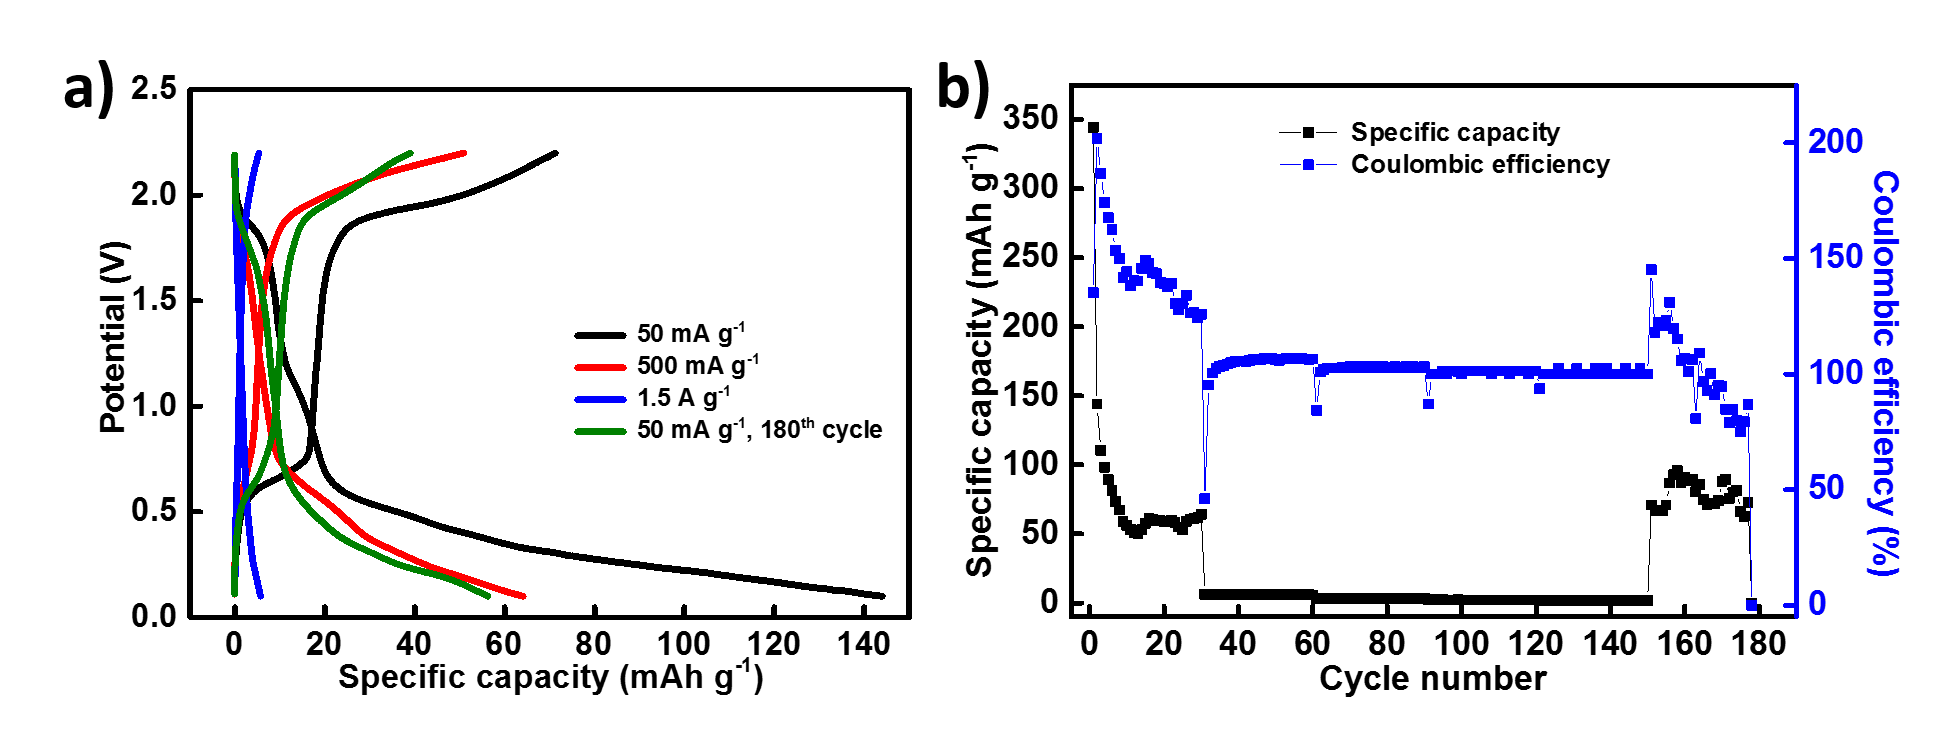
\includegraphics[width=\textwidth]{Figures/chap6fig/pbCDC2}
    \caption{Galvanostatic cycle test of an Al/\ce{C19Fe7N18}, Prussian blue, cell in a two-electrode setup at various current rates.}
  \label{Figures/chap6fig:pbCDC2}
\end{figure}

\subsection{Conclusion and future outlook}
In other battery systems, it had been reported that due to structure degradation, MOFs underwent large irreversible capacity losses and completed lesser number of cycles. This might be one of the reasons why the Al/MOF cell displayed a similar trend. However, Wang \ce{et al.} proposed a number of possible solutions to improve the performance of MOFs as a battery material. Supposing that the cell undergoes conversion-type reaction, the type of ligand in the MOF plays an important role because it determines if the MOF structure can be easily regenerated after every cycle. In case the cell undergoes an intercalation-type mechanism, MOF with a robust structure is highly desirable. A metal ion with multiple valence states and low molecular weight ligands rich in functional groups promotes insertion of \ce{Li+} ions \cite{wang_metalorganic_2016}. Therefore, altering the current MOF i.e. \ce{C19Fe7N18}, using the above-mentioned techniques would certainly improve its performance in AIBs. 
